\documentclass[journal,compsoc]{IEEEtran}
\usepackage[T1]{fontenc}
\usepackage[utf8]{inputenc}
\usepackage{amsmath,amssymb}
\usepackage{bm}
\usepackage{graphicx}
\usepackage{booktabs}
\usepackage{multirow}
\usepackage{array}
\usepackage{xcolor}
\usepackage{tikz}
\usetikzlibrary{arrows.meta,positioning,calc,fit,backgrounds,shapes.geometric,patterns}
\usepackage{pgfplots}
\pgfplotsset{compat=1.17}
\usepackage{algorithm}
\usepackage{algpseudocode}
\usepackage{listings}
\lstdefinestyle{code}{basicstyle=\ttfamily\scriptsize,breaklines=true,frame=single,framerule=0pt,rulecolor=\color{black!30},columns=fullflexible,keepspaces=true,aboveskip=3pt,belowskip=3pt}
\lstset{style=code}
\usepackage{mathtools}
\usepackage{amsthm}
\newtheorem{property}{Property}
\usepackage[hidelinks]{hyperref}
\usepackage{xurl}
\usepackage{enumitem}
\usepackage{xspace}
\usepackage{balance}
\setlist{itemsep=1pt,topsep=2pt}
\setlength{\textfloatsep}{5pt plus 1pt minus 2pt}
\setlength{\floatsep}{4pt plus 1pt minus 2pt}
\setlength{\intextsep}{5pt plus 1pt minus 2pt}
\def\SPSubmission{}

\graphicspath{{../figures/}}

\newcommand{\system}{RAGIN\xspace}
\newcommand{\RAGIN}{RAGIN\xspace}
\newcommand{\attck}{ATT\&CK\xspace}
\newcommand{\eg}{e.g.,\xspace}
\newcommand{\ie}{i.e.,\xspace}
\newcommand{\etal}{et al.\xspace}

\begin{document}

\title{The Intelligence Ladder: Pricing AI Capabilities in a Verified-Serving Deception Honeypot}
\author{Anonymous~Submission\thanks{Manuscript submitted to IEEE Transactions on Dependable and Secure Computing. Artifact, preregistration documents, and analysis code available at the anonymized repository upon acceptance.}\thanks{This work was conducted on infrastructure owned and operated by the authors. No external funding was received. The authors declare no conflicts of interest.}}
\maketitle

\begin{abstract}
How much intelligence can a deception endpoint spend crafting its lie before
that intelligence becomes the risk? We
study it with RAGIN, a verified deception loop in which retrieval-grounded
generation proposes a response, a fiction graph and deterministic checks
decide whether it may be served, and vetted content is the fail-safe. No
generative honeypot to date states a serving contract for its model's
output; RAGIN's contribution is that contract, and a ladder analysis that
prices every intelligence rung against its cheapest certifiable
competitor. A paired
90-scenario ablation reports that grounding lifts the analysis-channel
technique detection by $+0.317$ (95\% CI $[+0.162,+0.480]$) and actor
attribution by $+0.140$ ($[+0.083,+0.197]$) while persona realism is
unchanged; a fresh live-model rerun and a checkpoint-disjoint juror
confirm the differential is keyword matching, not substantive CTI
quality---the analysis channel prices retrieval, it does not measure
served deception quality.
On the served-text channel we report no capability gain: an echo-guarded audit
of our scorer invalidates the raw numbers, zeroing 97 of 218 rows. Verification
is measured where drafts violate the fiction: across 778 drafts from three
author families the serving path rejected 554 of the 572 invariant-violating
drafts and admitted 18 while refusing 17 of 206 benign ones. Purpose-built probes bound
the gate: it stops six of seven fluent, tell-free cases and all ten credential
formats after repair, but misses both prompt-injection cases; exposure to a real
credential is thus bounded by canary-registry discipline, not the verifier. In a paired thirty-turn adversarial workload under a pre-registered
protocol, five attacker personas drive both surfaces over SSH to the
turn cap: no persistence or bait-capture effect is measurable, and the
one separating interval---planted artifacts returned on adversarial
reads---replicates confirmatorily under a family-disjoint attacker
brain (6/10 versus 0/10, $p=0.011$; risk difference $0.60$, CI
$[0.30, 0.90]$), and a direct control shows stock cowrie's static
filesystem cannot serve planted files without restart---the contrast
measures dynamic serving capability stock surfaces structurally lack. A disclosed
three-checkpoint panel within one model family---machine labels, not
human ones---scores 120 cases at Fleiss $\kappa=0.81$. The result is a measured boundary around
generative deception: grounding buys intelligence the analysis channel
keeps, the gate bounds what may be served and publishes its own misses,
and the deterministic floor absorbs everything the model cannot
certify.
\end{abstract}

\begin{IEEEkeywords}
Cyber deception, honeypots, retrieval-augmented generation, large language
models, MITRE \attck, verified serving.
\end{IEEEkeywords}

\section{Introduction}
\label{sec:intro}

An attacker who has just landed inside a honeypot issues a single
request: \emph{show me the database credentials}. What the honeypot does
next divides two decades of deception engineering from the problem this
paper addresses. A recorder cannot answer at all; it writes the request
to disk and waits. A scripted honeypot answers from a file, the same file
for every attacker, on every visit, forever. A generative honeypot drafts
an answer on the spot---and the attacker may act on it, carrying it into
a timeline a security operations center will later treat as evidence. A
drafted credential exists nowhere except in the attacker's hands, and
nothing downstream can tell it apart from a secret that leaked; an
echoed real one converts the trap into a breach. The moment a honeypot
begins to answer it has taken on three jobs at once: stay consistent
with everything it has said, leak nothing real, and remain available
when the model behind it is not. A recent survey of production deception frameworks
identifies a gap in the surveyed systems: responses are not grounded in
real-time threat intelligence and behavior is not differentiated across
attacker classes~\cite{lopez2024}.

The cost of that silence is measured elsewhere: mean time to identify a
breach runs in months~\cite{ibm2024} while adversary breakout time has
compressed to minutes~\cite{crowdstrike2026}. A honeypot sits directly in
the attacker's path yet converts none of that proximity into
tactics-and-techniques intelligence a security operations center could act
on.

Large language models (LLMs) promise to close this gap. Prompted with a
session transcript and a library of threat intelligence, a modern LLM can
impersonate a vulnerable Linux host, improvise plausible file systems, and
steer the conversation toward the attacker's next objective. Recent systems
have begun to exploit this, deploying LLM agents as honeypots that chat an
attacker through a fictitious machine~\cite{reworr2024}. The promise,
however, arrives with a problem the deception literature has largely left
unexamined: \emph{the model can be wrong in ways a script cannot}. A
honeypot's product is a lie, and the lie must satisfy three properties at
once. It must be \emph{consistent}: the kernel version printed on turn one
cannot contradict the one an attacker reads on turn five, and the database
banner cannot disagree with the port the same host just advertised. It
must be \emph{safe to serve}: a model that complies too well will invent
credential material with no way to distinguish what it fabricated from
what it leaked, poisoning every downstream analytical product. And it
must be \emph{available}: a generator is a rented service, and ours was.
Operational traces in this study show catalog drift, quota exhaustion,
gateway outages, and safety-alignment refusals. Unverified generation can
forfeit all three properties in the same session.

The alternative---fixing the problem inside the model---fails on
inspection: prompting, refusal training, and constrained decoding shape
probabilities, but none can certify a particular output. Alignment
training produces refusal behavior that shifts with phrasing and
pressure~\cite{ganguli2022,bai2022}; our quota cliff exposed the same
failure under production conditions. And a deceived honeypot is itself an
LLM application with attacker-controlled context, so injection
techniques~\cite{greshake2023} apply with the attacker already in the
room. A probability, however small, is not a promise a security tool can
serve on; the assurance has to live outside the model.

The classical system-side fixes fail differently. Pre-scripting every
answer regresses to the finite automaton of low-interaction deception,
discarding the adaptivity that motivated generation in the first place;
real-time human review of every response cannot keep pace with an
attacker who reads faster than an analyst can vet. What survives is an
asymmetry between the two halves of the problem. Generating a plausible
answer to an arbitrary question is open-ended: its output space cannot
be enumerated, so no amount of testing certifies the next draw.
Checking a draft against a small, closed set of claims is the opposite:
a bounded computation whose verdict is final. A system can exploit this
by splitting the roles, letting the generator propose and a verifier
dispose against a fiction the system itself fully controls.

This paper takes the position that the right question is not
\emph{can an LLM impersonate a host} but \emph{how much intelligence can
a lie safely spend, and where must the spending stop}. Deception systems
build intelligence in rungs -- templates, classifiers, retrieval, free
generation -- and each rung has a trust price that practice pays
implicitly. We make the pricing explicit. Our answer is a verified
deception loop in which
each mechanism exists to buy one of the three properties, placed on a
single axis of certifiability (\S\ref{sec:ladder}). A fiction graph
binds every host fact to one consistent set of triples, and a verifier
checks every draft against that graph before anything reaches the wire:
consistency, enforced at serving time, not asked for at prompt time.
Baited content is drawn only from canary-registered secrets, so that any
disclosure is a measured event rather than a leak: safety by
construction. A deterministic fallback serves human-vetted transcripts
whenever generation or verification fails, so the system degrades to the
last known good answer rather than an unverified improvisation:
availability under provider failure. Beneath these sit a behavioral
profiler and a hybrid retrieval engine that ground a per-attacker
deception plan in curated CTI, giving the lie its targeting, and a
human-in-the-loop gate holds back any content class marked as requiring
approval. The loop turns generation from an act of trust into a measured
pipeline with an audit trail, and the evaluation reads the whole
apparatus as an escalation study: each rung of intelligence is measured
for what it adds over the rung beneath it, including the rungs that fold
back down when a certifiable mechanism reproduces their effect.

We evaluate whether each element of this loop contributes measurably,
using
artifact-backed benchmarks that we release alongside the paper. Four
questions structure the study:
\begin{itemize}
\item \textbf{RQ1:} Does retrieval grounding change CTI analysis, and
separately what is served? A paired ablation across 90 matched scenarios
reports grounding lifts analysis-channel technique detection by $+0.317$
(95\% CI $[+0.162, +0.480]$) and actor attribution by $+0.140$
($[+0.083, +0.197]$), leaving persona realism untouched---a null the
architecture predicts; the served-text comparison is reported separately,
never causally.
\item \textbf{RQ2:} Can an LLM-driven honeypot remain internally
consistent and safe under adversarial interaction? Across 45 targeted
re-queries the fiction graph serves zero contradictions; across a
218-query campaign the verification layer records no unverified response
served; and three authored model families expose bounded
precision/recall gaps.
\item \textbf{RQ3:} Is the resulting deception strong enough to hold a
skilled observer? A three-evaluator consensus study (independently
prompted LLM reviewer personas sharing one judge model) scores the full
session transcripts at $3.86/5$ with exact agreement $0.750$, all eight
scenarios at or above the acceptance bar, and a known judge bias
corrected by canary-registered secrets.
\item \textbf{RQ4:} Does each additional rung of intelligence justify its
trust price? The escalation analysis adds each mechanism to the same loop
and prices its marginal effect: on one 400-session held-out split the
profiler scores $0.8875$ as a whole-session classifier and $0.955$ when
the trajectory replay exposes each session's full command history---the
same corpus under two procedures, not an intervention delta; grounding
contributes the $+0.154$ comparison above; and kind-aware classification corrects 12/13 Cowrie-log assessments and
lifts bait exposure 125\% in five replays yet adds no measurable dwell
and is subsumed by a deterministic floor---a fold-down signal turning the
ladder into a design rule. A second pre-registered contrast on the serving surfaces---the first
between deception surfaces, to our knowledge---repeats the discipline:
both arms saturate the thirty-turn cap (log-rank $p=0.975$) and bait
capture is zero in both; the one separating interval (planted artifacts on adversarial reads,
11/20 versus 0) was promoted to the primary endpoint of a third
pre-registered contrast with a family-disjoint brain and replicated
confirmatorily (6/10 versus 0/10, $p=0.011$).
\end{itemize}

\noindent Our contributions are:
\begin{itemize}
\item \textbf{A verified deception architecture} (\S\ref{sec:design})
coupling RAG-grounded generation to a fiction graph and a serving-time
verification gate with deterministic fallback: every response is verified
against the deception state or drawn from vetted content.
\item \textbf{An archived analysis-channel grounding comparison}
(\S\ref{sec:evaluation}): paired-difference bootstrap intervals over
identical 90-row scenario sets report $+0.154$ overall improvement
($[+0.092, +0.221]$), with 35 TTP detections spanning 21 distinct techniques
versus zero without grounding. No clean served-text causal gain is claimed:
our own scorer audit yields echo-corrected lower bounds of 0.479 technique
and 0.243 actor for the archived campaign.
\item \textbf{A consistency and safety benchmark} (\S\ref{sec:evaluation}):
contradiction-free serving under adversarial re-query, a supported-claim
gate, a 105-case deterministic suite, a cross-family stress test, and an
ablation battery in which removing each mechanism (A1--A4) costs the
property it was added to provide.
\item \textbf{Run-to-run stability}: two archived 218-query reruns
reproduce the composite to $+0.005$ with $0.991$ per-row pass agreement
and exact deterministic-strata reproduction.
\item \textbf{A release package} on commodity hardware
(2~vCPU, ${\sim}4$~GB RAM), in which every headline number resolves to a
persisted result file, published on artifact acceptance.
\item \textbf{An escalation methodology for AI in deception}
(\S\ref{sec:ladder}, \S\ref{sec:jeveval}): mechanisms placed on a
certifiability axis, each rung priced by measured marginal effect under
pre-registered protocols, and the descent direction exercised on live
machinery -- when a certifiable mechanism reproduces an intelligent
one's benefit, the intelligent rung is removed from the ladder; a frozen
candidate that added no value beyond the gate on a prospective 40-case
cohort was retained disabled rather than claimed.
\end{itemize}

We are careful about what this paper does not claim. The deployment is
tailnet-only; the evaluation judge shares a provider with, but is a
different model from, the generator; the only labeling lane in this
release is the disclosed AI panel of \S\ref{sec:labels}; and the
full-system study that exercises the actual serving path ran in
deterministic provider-unavailable mode only. The threat model excludes
host compromise, provider compromise, and operator collusion, and the
closed command surface does not establish open-world robustness. These
limits are quantified where they arise (\S\ref{sec:threat-model},
\S\ref{sec:conclusion}).

Section~\ref{sec:threat-model} fixes the threat model and claim
boundary; \S\ref{sec:design} presents the loop; \S\ref{sec:related}
positions it; \S\ref{sec:evaluation} reports the battery, ablations, and
stability runs; \S\ref{sec:conclusion} concludes.

\section{Background and Threat Model}
\label{sec:threat-model}

\subsection{The Intelligence Ladder: Trust Prices and Exit Ramps}
\label{sec:rungs}

The design question this paper asks is how much intelligence a serving
loop should spend. We answer it with a pricing rule: a capability is
admitted to the serving path only if its measured marginal benefit
(\S\ref{sec:evaluation}) justifies its \emph{trust price} --- the
attack surface it opens, the certification burden it places on
everything downstream of it, and the availability dependency it
introduces. The loop answers the spending question with a single axis,
\emph{certifiability} --- whether a mechanism's output can be checked
against the closed world before it reaches the wire --- and spends
along it in rungs that compose: the ladder of \S\ref{sec:ladder}.
Table~\ref{tab:rungs} prices the four rungs the system implements and
declares each rung's \emph{exit ramp}: the deterministic behavior the
loop takes when the rung fails, so that no failure mode of any rung is
left to improvisation.

\begin{table}[t]
\centering
\caption{The four rungs of the intelligence ladder: what each
delegates to a less certifiable mechanism, its trust price, and its
declared exit ramp.}
\label{tab:rungs}
\scriptsize
\setlength{\tabcolsep}{2.5pt}
\begin{tabular}{p{0.13\columnwidth}p{0.31\columnwidth}p{0.45\columnwidth}}
\toprule
Rung & Decision delegated & Trust price and exit ramp \\
\midrule
R0 templates & none: serving itself & No intelligence to price; the floor that every other rung's exit ramp lands on (\S\ref{sec:fallback}) \\
R1 classifier & which deception policy a session receives & Cheap, deterministic at inference, auditable offline; a misroute changes what is served, never whether it is verified, and the deterministic behavior floor subsumes adaptive rerouting at $\Delta{=}0$ (\S\ref{sec:jeveval}) \\
R2 retrieval planner & which intelligence shapes the plan & Statistics over an open corpus upstream of the gate; failed or refused retrieval degrades the plan, never the serving rule (\S\ref{sec:don}) \\
R3 generator & what text to serve & The only rung not certifiable in advance; exit: one violation-fed retry, then R0, with \textsc{require} content stopping at the human gate (\S\ref{sec:verify}, \S\ref{sec:hitl}) \\
\bottomrule
\end{tabular}
\end{table}

The rule cuts in both directions: intelligence is admitted at a known
price, and a rung whose measured benefit can be reproduced by a
cheaper, certifiable mechanism should be compiled down.
\S\ref{sec:design} gives the mechanism and the descent;
\S\ref{sec:evaluation} gives each rung's measured marginal.

\subsection{Threat Model}

We consider an attacker who may observe and re-query a session, start
fresh sessions, inject instructions through commands or retrieved
content, submit malformed or high-rate input, and adapt to previously
observed verifier behavior. Cross-session probing, provider refusal,
and retry pressure are in scope. A compromised host, container escape,
provider-side compromise, and operator collusion are outside the
in-system security property: they are deployment prerequisites rather
than properties certified by the verifier.

\begin{table*}[t]
\centering
\caption{Attacker capabilities, the property each pressures,
evaluation status with its evidence, and explicit nonclaims. All
evidence is bounded to the named workload or declared command surface.}
\label{tab:capability}
\scriptsize
\setlength{\tabcolsep}{3pt}
\begin{tabular}{p{0.15\textwidth}p{0.14\textwidth}p{0.31\textwidth}p{0.30\textwidth}}
\toprule
Attacker capability & Pressures & Evaluation status (evidence) & Explicit nonclaim \\
\midrule
Observe, re-query, adapt: cross-referencing turns, fresh sessions,
identity or consistency drift, degenerate-output probes. An injected draft that stays on-fiction and identity-correct passes by
construction; containment is the fiction graph's blast radius---a
poisoned plan alters one session's facts and is re-seeded at next
contact, never prior sessions (\S\ref{sec:hostfiction}) &
Fail-closed serving &
105-case verifier suite; 778 induced drafts from three author families
of which the serving path rejected 554 of the 572 violating drafts and
admitted 18, refusing 17 of 206 benign; 45 graph re-queries; boundary
probes stopping 6 of 7 authored disclosures and all 10 credential
formats after the round-2 repairs (4 of 7 and 5 of 10 pre-repair;
\S\ref{sec:rq2}) &
Not open-world resistance, realism, or coverage against arbitrary
adaptive drafts. A fluent, on-fiction secret disclosure is not detected
in general: exposure to a real credential is bounded by canary-registry
discipline, not by the verifier. \\
Supported-claim completeness on the declared eight-command surface
(\texttt{whoami}, \texttt{id}, \texttt{hostname}, \texttt{uname},
\texttt{echo}, \texttt{uptime}, \texttt{date},
\texttt{cat} of \texttt{/etc/os-release}) &
Supported-claim completeness &
123 supported-claim cases over exactly that surface &
Closed-surface recall only; no general semantic guarantee. \\
Instruction injection through commands or retrieved content &
Targeted scoring of the gate &
Two induced-draft cases; both carry targeted-scoring misses; one
variant of one case passed the gate &
Injection resistance is not credited anywhere in this paper, and no
injection-robustness wording appears in the property set. \\
Influence the CTI corpus: poisoning, stale or adversarial corpus rows &
Grounding; corpus screening &
Screening and quarantine mechanisms exist in the ingestion path;
retrieval-removed comparison on the same fixed scenario set with
paired bootstrap: $+0.154$ composite ($95\%$ CI $[+0.092,+0.221]$),
archived and model-coherent &
Retrieval poisoning is not adversarially evaluated; the grounding
comparison is not a clean served-text causal result, and fresh
reproduction remains external work. \\
Carry state across sessions or hosts &
State isolation &
Host-fiction and graph-consistency artifacts, including 4/4
deterministic cross-session drift cases &
No multi-tenant or compromised-host guarantee. \\
Malformed, empty, or non-shell output; high-rate queries, large
payloads, retry amplification &
Fail-closed degenerate handling; availability &
Degenerate cases in the verifier battery; deterministic fallback and
offline failure-path battery &
No field-load availability, cost, or tail-latency claim. \\
Provider refusal, timeout, quota exhaustion, catalog churn &
Availability &
The full failure taxonomy observed across this project's deployments;
fallback serves the deterministic floor &
Provider-side compromise and provider trust are out of scope;
availability degrades to R0 and no further provider property is
claimed. \\
Manipulate the evaluation judges (LLM-as-a-judge channel) &
Measurement integrity &
Judges treated as measurement instruments: results labeled by who
judged, guarded rubric, blinded echo audit, deterministic strata &
Bound, not eliminated: no LLM judge is a serving-time security
control; serving-contract evidence is deterministic and reported
separately (\S\ref{sec:evaluation}). \\
\bottomrule
\end{tabular}
\end{table*}

The trusted computing base is the deterministic verifier, the
fiction-graph state and its isolation boundary, the canary registry,
vetted fallback transcripts, the gateway's key and retry policy, and
the append-only audit record. The LLM, retrieved CTI, attacker input,
and provider availability are untrusted or unreliable inputs. The
serving claim is deliberately narrow: a draft is served only when it
passes the declared checks, otherwise the system falls back or stops at
the human gate. Defenders operate the system within policy: the human
gate exists because some content classes should not be served without
a human decision, even when the machinery would allow it.

The evaluation channel is modeled as attackable rather than as ground
truth. The judges that score deception quality in
\S\ref{sec:evaluation} err on hard objective tasks~\cite{tan2025judgebench},
and attacker-controlled inputs can manipulate the judge
itself~\cite{shi2024judgedeceiver}; ours share a provider with the
generator (different family), a common-mode risk that the consensus
protocol and rubric corrections bound but do not eliminate, and a
realized scoring attack --- our own scorer crediting echo text as
grounded content --- was caught by the blinded audit, whose guarded
rubric replaces it. The consequence is architectural: every LLM judge
here is a measurement instrument, never a serving-time security
control, matching the exact-oracle preference of agent-evaluation
practice~\cite{debenedetti2024agentdojo}; serving-contract evidence,
deterministic and replayable, is reported separately from judge-scored
behavioral metrics, each result labeled by who judged it. That is why
the judge row of Table~\ref{tab:capability} reads \emph{bound, not
eliminated}.

The held-out rescue benchmark and the adaptive ladder are treated as
exploratory controller diagnostics. The rescue risk floor is derived
from the controller itself, and the ladder's five-pair replay has no
power to establish attacker engagement or security benefit.

Two capabilities above are declared in scope but unevaluated beyond
what their rows record: instruction injection carries targeted-scoring
misses with a passing variant, and retrieval poisoning is not evaluated
at all. The verifier is therefore not credited with injection
resistance anywhere in this paper, and no poisoning-resistance wording
appears. Table~\ref{tab:capability} is the claim boundary the evidence
supports; stronger claims require independently constructed attacks,
independent quality evaluation, or field deployment.

\section{The Verified Deception Loop}
\label{sec:design}

\RAGIN is organized around one invariant: \emph{nothing is served that has
not been either verified against the session's deception state or produced
from vetted deterministic content}. Three design decisions give the
invariant its shape, each chosen against an alternative that fails in an
instructive way.

First, verification is post-hoc. The obvious alternative is to constrain
generation itself: constrained decoding, grammar templates, or output
licenses. Such mechanisms bound the \emph{shape} of an output, but the
properties that matter here are semantic (does this banner agree with the
port from turn one?), and a promise about the process is not a
certificate about the artifact. A draft must be judged on what it says,
which is only possible after it exists; hence draft, then check.

Second, the check runs against a \emph{graph}, not against the prompt or
the transcript. \S\ref{sec:intro} argued the asymmetry: an arbitrary
answer has an unenumerable output space, but a closed world of committed
facts is small enough to check exhaustively. The fiction graph is that
closed world. Its smallness is the design's load-bearing property: it
makes verification a bounded computation with a final verdict rather
than another probabilistic judgment in need of a judge.

Third, the graph's lifetime is the session. A per-session fiction bounds
the blast radius of any drift or poisoning to one attacker's view, and an
attacker who returns presents a fresh world rather than an accumulated
liability. Cross-session continuity is a separate, host-keyed layer
described in \S\ref{sec:hostfiction}: the implementation additionally
maintains attacker-level behavioral memory in the deployed stack, and
unifying the two memory planes further
is future work (\S\ref{sec:conclusion}), not a hidden coupling.

The mechanisms below hold five goals, each naming the failure it
prevents, its enforcing component, and its falsifying measurement:
\begin{itemize}
\item \textbf{G1 (Grounding).} Deception is conditioned on who the
attacker is and on current threat intelligence---preventing irrelevant
deception no attacker class finds plausible; enforced by the profiler and
retrieval planner, measured by the paired grounding differential.
\item \textbf{G2 (Consistency).} Every observable artifact resolves to one
set of facts---preventing inconsistency as an information channel to a
re-querying attacker; enforced by the fiction graph and the verifier,
measured by contradiction rate under re-query.
\item \textbf{G3 (Safety).} No unverified content reaches the wire and
dangerous classes require human approval---preventing over-disclosure;
enforced by the verifier, canary registration, and the HITL gate,
measured by verified-serve rate and gate audit coverage.
\item \textbf{G4 (Graceful degradation).} On generation, verification, or
provider failure the loop serves deterministic vetted content---preventing
unverified improvisation under outage; enforced by the deterministic
fallback, measured by fallback correctness and serve-path provenance.
\item \textbf{G5 (Attribution).} Every decision leaves an audit trail
sufficient to reconstruct why a response was served---preventing
undebuggable behavior; enforced by serve-path provenance labels, measured
by the audit census of \S\ref{sec:evaluation}.
\end{itemize}
G5 is not a logging feature: it makes the other four falsifiable, and a
verification gate that does not persist its rejections can be believed,
not audited --- so the evaluation treats the audit trail as primary
evidence rather than instrumentation.

This section walks the loop in serving
order. Figure~\ref{fig:architecture} gives the overview; each subsection
names the goal that the component exists to satisfy.

\subsection{The Intelligence Ladder}
\label{sec:ladder}
Every mechanism in the loop is an instance of one decision: how much
intelligence to spend on the deception, and where the spending stops.
\S\ref{sec:rungs} prices that decision --- the trust price and declared
exit ramp of each rung on the certifiability axis; this subsection is
the mechanism that makes the pricing enforceable: the rungs as they
run in the loop, each with its measured effect
(\S\ref{sec:evaluation}):

\begin{itemize}
\item \textbf{R0, deterministic templates} (the fallback,
\S\ref{sec:fallback}): no intelligence, consistency by
construction, zero adaptation. This rung defines the system's floor
under failure and doubles as the control condition: ablation A5 checks that the
loop degrades to it safely, verified and serving, when the graph engine
does nothing.
\item \textbf{R1, behavioral classification} (Chrollo,
\S\ref{sec:chrollo}): low-cost routing decisions over session
features -- auditable, offline, deterministic at inference. Measured
marginal: held-out classification accuracy 0.8875 $\to$ 0.9550 with
n-gram features; a routing-accuracy ladder of its own
(\S\ref{sec:jeveval}).
\item \textbf{R2, grounded planning} (Don, \S\ref{sec:don}):
retrieval-augmented generation over curated CTI. Measured marginal: the
paired $+0.154$ composite grounding effect with 35 TTP detections
spanning 21 distinct techniques, versus zero without grounding (RQ1) -- real adaptive value, but each output remains a
statistic over an open corpus.
\item \textbf{R3, free generation under verification} (the generator
plus verifier, \S\ref{sec:verify}): the only rung whose output cannot be
certified in advance, admitted solely because the verifier converts its
artifacts into checked facts at serving time or the fallback catches
what verification rejects.
\end{itemize}

\noindent Figure~\ref{fig:ladder} renders the ladder with each rung's
measured marginal effect at its side.
The ladder runs in both directions, which makes it a design
model rather than a build history. Escalating buys capability at
a known trust price; \emph{descending} is the load-bearing direction: a
rung that can be compiled down -- replaced by a cheaper, certifiable
mechanism that reproduces its measured benefit -- should be. The routing
arm of \S\ref{sec:jeveval} shows the descent directly: an LLM
kind-assessment rung that historically fixed 44/44 misrouted sessions was
subsumed by a deterministic behavior floor at zero marginal accuracy --
the final held-out comparison scores both arms 200/200, with no
assessment output available on any session (\texttt{jev\_available}$=0$)
-- and the floor needs no network, no provider, and no trust.
Intelligence past the point
where a certifiable mechanism reproduces its effect is not an asset; it
is an attack surface with a quota bill.

% The intelligence ladder: four rungs on the certifiability axis, each
% with its measured marginal effect, and the measured fold-down from the
% top rung to the deterministic floor. Rendered from the persisted
% artifacts cited in the rung labels; all values are hardcoded here only
% because the figure must compile without the results directory.
% Geometry note: the fold-down curve is routed through the corridor left
% of the stack (control x = -3.45; every rung box edge is at x >= -2.8),
% and the stack arrows run rung-to-rung with no intervening text, so no
% arrow segment crosses a node or label interior.
% GENERATED by scripts/gen_sp_figures.py -- do not edit by hand.
% Every plotted number in the S&P figures resolves through this file, so a
% figure cannot silently disagree with the artifact it claims to show.
% Regenerate:  python scripts/gen_sp_figures.py
% Verify:      python scripts/gen_sp_figures.py --check
% Sources:
%   results/bootstrap_ci.json
%   results/stability_run1_vs_run2.json
%   results/b4_baseline_zodiac_20260922.json
%   results/model_quality/chrollo_calibration.json
%   results/sp2027_rescue/behavior_trajectory_benchmark.json

\def\RaginLiveTechnique{0.9598}
\def\RaginLiveTechniqueErrLo{0.0122}
\def\RaginLiveTechniqueErrHi{0.0122}
\def\RaginLiveActor{0.8500}
\def\RaginLiveActorErrLo{0.0000}
\def\RaginLiveActorErrHi{0.0000}
\def\RaginLivePersona{0.7325}
\def\RaginLivePersonaErrLo{0.0587}
\def\RaginLivePersonaErrHi{0.0558}
\def\RaginLiveComposite{0.8796}
\def\RaginLiveCompositeErrLo{0.0224}
\def\RaginLiveCompositeErrHi{0.0204}
\def\RaginLivePersonaRunTwo{0.7504}
\def\RaginLiveCompositeRunTwo{0.8845}
\def\RaginPersonaRunDelta{0.018}
\def\RaginTechDelta{0.317}
\def\RaginTechDeltaLo{0.162}
\def\RaginTechDeltaHi{0.480}
\def\RaginActorDelta{0.140}
\def\RaginActorDeltaLo{0.083}
\def\RaginActorDeltaHi{0.197}
\def\RaginPersonaNullDelta{0.005}
\def\RaginPersonaNullDeltaLo{-0.047}
\def\RaginPersonaNullDeltaHi{0.057}
\def\RaginOverallDelta{0.154}
\def\RaginOverallDeltaLo{0.092}
\def\RaginOverallDeltaHi{0.221}
\def\RaginGroundingTtpCount{35}
\def\RaginNoGroundingTtpCount{0}
\def\RaginRoutingBefore{0.8875}
\def\RaginRoutingAfter{0.955}

\begin{figure}[t]
\centering
\begin{tikzpicture}[
  font=\scriptsize,
  rung/.style={draw, rounded corners=1pt, thick, align=center,
               inner sep=2.5pt},
  floor/.style={rung, fill=black!12},
  gen/.style={rung, fill=black!4},
  removed/.style={rung, draw, dashed, fill=none, text=black!60},
  arr/.style={-{Latex[length=1.6mm]}, semithick},
  darr/.style={-{Latex[length=1.6mm]}, semithick, dashed}
]
  % ── rungs: mechanism on the first line, measured effect beneath it ──
  \node[removed] (r4) at (0,5.85) {kind-aware assessment
        \;{\tiny(assessed, removed)}\\
        {\tiny\itshape no marginal effect resolvable at the benchmark's ceiling}};

  \node[gen] (r3) at (0,4.05) {R3\; free generation under verification\\
        {\tiny\itshape adaptivity; 0 unverified serves across 218 queries}};

  \node[gen] (r2) at (0,2.25) {R2\; grounded planning
        \;{\tiny(Don)}\\
        {\tiny\itshape $+\RaginOverallDelta$ composite $[+\RaginOverallDeltaLo,+\RaginOverallDeltaHi]$;\; \RaginGroundingTtpCount{} vs \RaginNoGroundingTtpCount{} TTPs}};

  \node[gen] (r1) at (0,0.45) {R1\; behavioral classification
        \;{\tiny(Chrollo)}\\
        {\tiny\itshape routing $\RaginRoutingBefore \to \RaginRoutingAfter$; milliseconds, offline}};

  \node[floor] (r0) at (0,-1.35) {R0\; deterministic templates
        \;{\tiny(fallback)}\\
        {\tiny\itshape consistency by construction; zero adaptation}};

  % ── the stack: each rung rests on the cheaper one below it ──
  \draw[arr] (r0) -- (r1);
  \draw[arr] (r1) -- (r2);
  \draw[arr] (r2) -- (r3);
  \draw[arr, black!60] (r3) -- (r4);

  % ── the fold-down: measured descent from the top back to the floor,
  %    routed through the empty corridor left of the stack ──
  \draw[darr, thick]
    (r4.west) .. controls (-3.45,4.6) and (-3.45,-0.6) .. (r0.west);
  \node[rotate=90, anchor=south, font=\tiny\itshape, text=black!60,
        align=center] at (-3.62,2.0)
        {fold-down: the floor reproduces the measured benefit at zero
         trust price};
\end{tikzpicture}
\caption{The intelligence ladder. Each rung is admitted only above the
certifiable rungs beneath it, and each rung carries its measured
marginal effect (\S\ref{sec:evaluation}). The dashed arrow is the
result RQ4 adds: the assessed kind-awareness rung descended to the
deterministic floor -- no effect the benchmark resolves, no regression
risk, no provider dependency. Descending is the load-bearing direction;
a rung that cannot show a measurable benefit above the rung below it
does not stay on the ladder.}
\label{fig:ladder}
\end{figure}

\begin{figure*}[t]
\centering
% \includegraphics[width=\textwidth]{fig_architecture.pdf}
% Verified deception loop architecture (single-column TikZ)
% Routing discipline: main path is a straight vertical spine; all side
% paths run orthogonally in dedicated corridors (left margin, right gap)
% and enter nodes at distributed anchors, so no line crosses a node or
% another arrowhead.
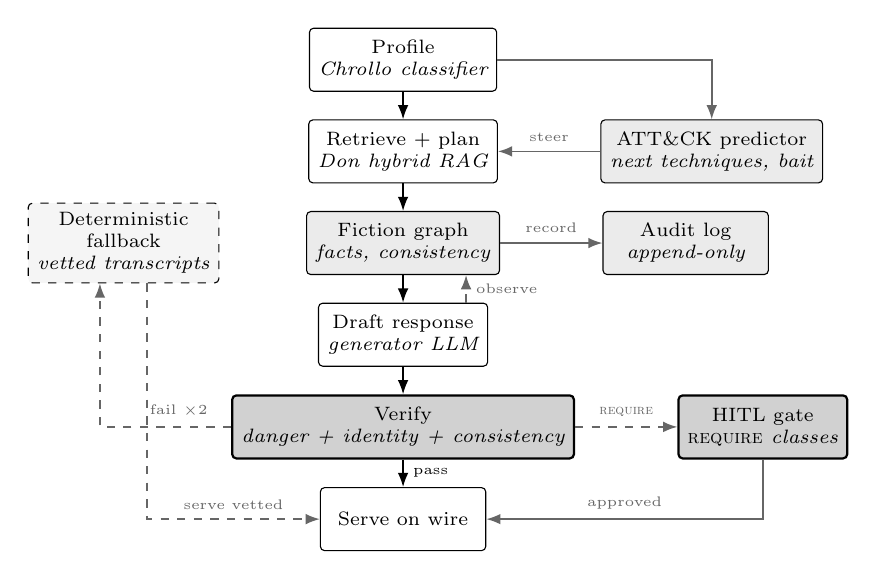
\begin{tikzpicture}[
  node distance=3.5mm and 5mm,
  stage/.style={draw, rounded corners=1.5pt, minimum height=8mm, minimum width=21mm, align=center, font=\scriptsize},
  store/.style={stage, fill=black!8},
  gate/.style={stage, fill=black!18, thick},
  fail/.style={draw, dashed, rounded corners=1.5pt, minimum height=8mm, align=center, font=\scriptsize, fill=black!4},
  arr/.style={-{Latex[length=1.8mm]}, semithick},
  farr/.style={arr, dashed, black!60}
]
% Main serving path (top to bottom)
\node[stage] (profile) {Profile\\ \scriptsize\itshape Chrollo classifier};
\node[stage, below=of profile] (retrieve) {Retrieve + plan\\ \scriptsize\itshape Don hybrid RAG};
\node[store, below=of retrieve] (graph) {Fiction graph\\ \scriptsize\itshape facts, consistency};
\node[stage, below=of graph] (draft) {Draft response\\ \scriptsize\itshape generator LLM};
\node[gate, below=of draft] (verify) {Verify\\ \scriptsize\itshape danger + identity + consistency};
\node[stage, below=of verify] (serve) {Serve on wire};

% Side stores
\node[store, right=13mm of retrieve] (mitre) {\attck predictor\\ \scriptsize\itshape next techniques, bait};
\node[store, right=13mm of graph] (audit) {Audit log\\ \scriptsize\itshape append-only};
\node[gate, right=13mm of verify] (hitl) {HITL gate\\ \scriptsize\itshape \textsc{require} classes};

% Failure path
\node[fail, left=11mm of graph] (fallback) {Deterministic\\ fallback\\ \scriptsize\itshape vetted transcripts};

% Main path arrows (vertical spine)
\draw[arr] (profile) -- (retrieve);
\draw[arr] (retrieve) -- (graph);
\draw[arr] (graph) -- (draft);
\draw[arr] (draft) -- (verify);
\draw[arr] (verify) -- (serve) node[midway, right, font=\tiny] {pass};

% Failure arrows: orthogonal, left corridor, offset anchors
\draw[farr] (verify.west) -| ([xshift=-3mm]fallback.south)
  node[pos=0.2, above, font=\tiny] {fail $\times$2};
\draw[farr] ([xshift=3mm]fallback.south) |- (serve.west)
  node[pos=0.75, above, font=\tiny] {serve vetted};

% Approval arrow: right corridor into serve.east
\draw[arr, black!60] (hitl.south) |- (serve.east)
  node[pos=0.75, above, font=\tiny] {approved};
\draw[farr] (verify.east) -- (hitl.west) node[midway, above, font=\tiny] {\textsc{require}};

% Feedback / context arrows: right gap, offset entry into graph.south
\draw[arr, black!60] (mitre) -- (retrieve) node[midway, above, font=\tiny] {steer};
\draw[arr, black!60] (profile.east) -| (mitre.north);
\draw[arr, black!60] (graph.east) -- (audit.west) node[midway, above, font=\tiny] {record};
\draw[farr] ([xshift=8mm]draft.north) -- ([xshift=8mm]graph.south)
  node[midway, right, font=\tiny] {observe};
\end{tikzpicture}

\caption{The verified deception loop. A session enters through the
behavioral classifier (Chrollo), which routes it to a per-class deception
policy. The retrieval engine (Don) grounds the policy in CTI; the fiction
graph binds every host fact; the generator drafts under the binding; the
verifier checks the draft against the graph before serving. Dashed paths
are failure paths: verification failure falls back to deterministic
transcripts, and content flagged \textsc{require} pauses at the
human-in-the-loop gate.}
\label{fig:architecture}
\end{figure*}

\subsection{The Fiction Graph}
\label{sec:graph}
Every fact the honeypot projects about itself (hostname, kernel, listening
ports, installed databases, user accounts) is stored as a
subject--predicate--value triple in a per-session \emph{fiction graph}.
The graph is seeded from the host identity at session start and grows by
two mechanisms: \emph{declaration}, when the deception plan asserts a new
fact, and \emph{observation}, when a served response is scanned and any
host-like entities it emitted are extracted and recorded. Observation is
the mechanism that binds the LLM to the recorded state: whatever the generator said the
host is, the graph now remembers, and the next draft must agree with it.

A triple carries its source, and consistency is checked at the predicate
level: two declarations of the same predicate with different values raise
a contradiction, with normalization tuned to distinguish a genuine
conflict from a benign surface variant (a hostname is not contradicted by
its fully qualified form). When a contradiction is detected, the graph
records it and the verification node treats any draft resting on the
contradicted fact as unservable. The fiction graph is what turns G2 from
an aspiration into a data structure; the serving-time invariant below
states the consistency condition it enforces and its attacker-visible
scope.

\subsection{Verified Generation}
\label{sec:verify}
Generation is a draft, not a decision. The generator (a provider-hosted
LLM) receives the session context, the deception plan, a compact
serialization of the fiction graph (a \emph{fact block}), and the
steering context: the \attck techniques predicted to follow the
attacker's observed sequence, together with bait artifacts matched to
those techniques. The prediction uses the \attck tactic ordering to
propose the attacker's likely next moves (G1's steering half).

Before a draft reaches the wire it passes five checks:
\begin{enumerate}
\item \textbf{Danger scan.} A pattern gate rejects credential-material,
offensive-content, and real-secret signatures; one considered exemption: a
bare token a real command would print (the correct answer to
\texttt{whoami} is one word) is not chatter.
\item \textbf{Identity pin.} Identity-revealing commands answer from the
persona's pinned identity---a novice never answers \texttt{whoami} with
\texttt{root}, the hostname never changes mid-session, a root-prompting
attempt is rejected. The C1 battery carries a dedicated proof.
\item \textbf{Consistency check.} Host-like entities are observed into the
fiction graph; a contradictory draft is rejected with the contradiction
recorded.
\item \textbf{Supported-claim check.} On the declared deterministic
command surface, the draft must \emph{contain} the correct
answer---hedging, echoing, or omitting is a rejection; outside the
declared surface the check is silent, so open-ended recall is untouched.
\item \textbf{Terminal sanity.} Shell-shaped responses that answer a
command with sentence-like prose instead of executable output are
rejected.
\end{enumerate}
A draft that fails any check is retried once with the violation fed back;
a second failure triggers fallback. The checks were selected by one
criterion: each must be a \emph{decision procedure} over the draft,
decidable, cheap, and deterministic, because a verifier that itself calls
a model would only relocate the trust problem it exists to solve. What
verification deliberately does not certify is quality. A draft can pass
all five checks and still be unpersuasive; plausibility is not
decidable, and the paper does not pretend otherwise. The division of
labor is the point: the loop's machinery enforces the three properties
of the three safety constraints machine-checkably, and the consensus study of
\S\ref{sec:rq3} assesses the deception quality that only evaluation can
measure. This is the mechanism behind the zero-unverified-serves claim
evaluated in \S\ref{sec:evaluation}. The serving sequence above gives
the full loop; its fallback arm carries G4 and its \textsc{Require}
branch carries G3.

\subsection{Cross-Session Host Fiction}
\label{sec:hostfiction}
The per-session fiction buys bounded blast radius
at a measured price: a returning attacker is shown a fresh world, and
none of the session verifier's checks can see drift \emph{between}
sessions. The host-fiction layer closes exactly that gap without
widening the blast radius. It is host-keyed rather than session-keyed:
at an attacker's first contact with a host, its identity is pinned and
provisioned into every consumer --- the persona prompt is rebuilt from
the pinned identity (removing a class of contradictory-instruction
failures where prompt and verifier disagreed), the session graph is
seeded authoritatively for verification, and the fallback template
inherits the same identity. Facts observed in a session are promoted to
the host store only when they passed verification (fail-closed: an
unverified session never binds a host fact), and every subsequent
session against the same host is cross-checked against the promoted
set by a session-verifier wrapper that rejects on cross-session
contradiction. Reconnect policies are configurable: a returning
connection can share the pinned graph outright, or start a promoted
session whose facts are cross-checked against the host.

The layer is measured, not merely present. On identical deterministic
drift scenarios (reconnect drift, beyond-identity drift, cross-skill
host swap, simultaneous contradiction, repetition controls), the
session-scoped verifier alone catches 1 of 4 cross-session drift drafts;
both host-fiction policies catch 4 of 4 with 0 of 7 benign re-query
false rejections (\path{cross_session_consistency_bench.json}). The
three misses of the session-scoped baseline are invisible to it by
construction --- facts asserted in a previous session simply are not in
current-session state --- and per-skill identities name different hosts,
so a reclassified returning attacker would otherwise be shown a
different machine. On benign traffic the layer is free: paired over the
full 218-query workload, store-on versus store-off serves byte-identical
strings on every row (paired per-row delta exactly $0.0000$;
\path{external_baseline_hostfiction_comparison.json}), so cross-session
consistency is added at zero quality cost on the evaluated surface.

\subsection{Human-in-the-Loop Gate}
\label{sec:hitl}
Content classes whose compromise value is high (deployed credentials,
for instance) are marked \textsc{require} in the deception policy. When a
response would serve such content, the loop pauses and the decision is
surfaced to the operator through an audit interface that records the
context, the draft, and the decision. Every gate decision is persisted to
an append-only audit log, which \S\ref{sec:evaluation} uses as a
correctness and governance record.
The gate encodes a governance position: the system may \emph{draft}
deception, but a human decides when the deception includes trap
material (G3). The gate exists for the operator's stake, not the
attacker's: canary bait is safe to serve by construction, but it is
still an active measure whose use an operator may be required to
authorize; the audit record of that authorization leaves the system
defensible after the fact. The require-level branch is also where the
credential-deployment decisions in the benchmark trail
(Appendix~\ref{app:audit}) were made.

\subsection{Deterministic Fallback}
\label{sec:fallback}
Every scenario class has a vetted deterministic transcript: hand-written,
fiction-consistent bait and response templates (credential hunts, service
enumerations, exfiltration decoys) whose secrets are registered canaries.
When generation fails, the provider times out, verification rejects twice,
or the model refuses the persona, the loop serves the deterministic
transcript for the scenario instead. The fallback is not an admission of
defeat; it is the safety floor that makes the LLM path safe to enable.
The A5 ablation checks that the system is \emph{equivalent} through the
fallback path, and the design of the canary registration is what allows
the consensus study to distinguish deployed bait from accidental leaks.

Session state beyond identity facts replays the same discipline. A
filesystem ledger records the bytes served for every read command and
replays them verbatim when the same path is read again; time-varying
ambient content (process identifiers, timestamps, clock outputs) is not
stored but generated by hashing a per-session seed through a template,
so re-reads are identical within a session while sessions differ
plausibly from one another, and a mutating command invalidates the
affected entries so subsequent reads reflect the mutation. This ledger,
not the generative path, is what the byte-identical replay component of
the C1 result (\S\ref{sec:rq2}) exercises: determinism on re-query is a
property of how session state is stored and replayed, and the design
keeps it decoupled from generation.
The fallback also carries a hidden load: it defines the system's floor
under failure. Because the fallback serves the same fiction the generator
would have, an attacker cannot distinguish a degraded session from a
healthy one by content alone; the availability
property of G4 thereby becomes a deception property, not merely a reliability one.
What the fallback gives up is the generator's adaptivity: a fallback
session answers within its scenario's script and steers no further,
which is the correct trade only because the loop treats it as a floor
beneath the LLM path rather than the path itself.

\section{Related Work}
\label{sec:related}

\subsection{Honeypots and Cyber Deception}

Surveys of large language models in security \cite{wang2024} and of cyber
deception specifically \cite{lopez2024} frame the opportunity and its open
questions. Honeypots have been studied as instrumentation for two decades
\cite{spitzner2002}, and their engineering trade-offs---visibility,
fidelity, and the operational cost of interaction---remain open
\cite{sokol2017}. Adaptive deception work formalizes the
defender's decision to engage, treating attacker intent as something to
infer and modulate, through factored interactive POMDPs
\cite{shinde2020}, engagement--yield models
\cite{bera2024}, and behavioral partitioning under cognitive load
\cite{liska2024}. Deception has also been embedded in higher-fidelity
simulation and emulation targets \cite{kouremetis2024}. We adopt as our
starting point the gap that deception-framework surveys identify in deployed
systems: that they neither ground responses in live threat intelligence
nor differentiate behavior across attacker classes \cite{lopez2024}. Our
contribution is orthogonal to that taxonomy. We do not propose a new
deception policy; we constrain what a generative policy is allowed to serve.

\subsection{Generative Honeypots}

The closest prior art puts a language model inside the deception endpoint.
LLM-in-the-shell honeypots make the model answer as a live machine
\cite{valeros2024}; LLM agent honeypots instead monitor autonomous AI
attackers in the wild \cite{reworr2024}; and recent systems extend
generative deception to industrial protocols and physical-process emulation
\cite{vasilatos2025llmpot}, coordinated IoT deception
\cite{guan2025cpds}, and directory services
\cite{jimenez2025}. Analysis pipelines over collected honeypot and
incident data apply generative or learned models after the fact, for attack
classification and reporting \cite{lanka2024,simoni2024,blefari2025},
structured CTI mapping \cite{orbinato2022}, and attack investigation
\cite{alsaheel2021}. In all of these systems the model's output is the product, and the
product ships unchecked. None of them states a serving contract for that
output---no fixed fiction to be consistent with, no deterministic gate
that can refuse a draft, no vetted answer to fall back to when the
provider refuses or times out. To our knowledge, that contract is what
this paper adds, together with the ladder analysis that prices it; the
generative mechanisms themselves are borrowed.

\subsection{Runtime Enforcement and Red-Teaming of LLM Applications}

The verifier is the closest analogue in prior art, and the analogy is
deliberate. AgentSpec provides runtime enforcement for LLM agents
\cite{wang2026agentspec}; prompt-injection defences that constrain
decoding rather than trusting a probability appear in
\cite{chen2025struq,chen2025secalign}; the injection threat is
formalized in \cite{greshake2023} and measured by AgentDojo
\cite{debenedetti2024agentdojo}; tool-bearing agents add cross-tool
harvesting \cite{li2026dissonances}; model-red-teamed evaluation is
standard practice \cite{ganguli2022,perez2022,bai2022,christiano2017}. Our design follows
that literature's premise that assurance must live outside the model. What
differs is the asset being protected. A guardrail protects the assistant's
user from the model's output; this gate protects the attacker's belief from
the fiction's, so the failure of interest is a fluent, self-consistent,
on-script response that is nonetheless wrong for the deception state, and
the mitigation is a deterministic fallback to vetted content rather than a
refusal.

\subsection{Retrieval Grounding, and the Attacks We Do Not Yet Resist}

Retrieval grounding supplies the targeting rung \cite{lewis2020};
retrieval for threat intelligence is well populated---technique
extraction \cite{fayyazi2023,lekssays2025}, knowledge-graph construction
\cite{gao2025,jeon2024,belmahjoub2025}, index families \cite{malkov2018}
we price against sparse retrieval, response assistants
\cite{rajapaksha2024,paul2025,qiao2025,liu2025}, and the \attck{}
grounding question \cite{roy2023,alsada2024,noureddine2020}. The
security of that retrieval layer is an active literature: vulnerability
identification \cite{xue2024,liang2025}, RAG threat vectors and
mitigations \cite{ward2025}, knowledge corruption
\cite{zou2025poisonedrag,chaudhari2024}, retrieval jamming
\cite{shafran2024}, poisoning evaluation \cite{malladi2026ripeii},
poisoning-aware CTI ranking \cite{jia2025}, and attribution for poisoned
knowledge \cite{zhang2026ragorigin}. We adopt that literature's threat
model as out of scope for demonstrated results: this paper evaluates no
retrieval poisoning and no injection defence, and
Section~\ref{sec:threat-model} records that as a gap. The retrieval layer
sits inside the threat surface this literature has already mapped, so a
deployment that inherits it inherits those attacks, and the grounding
rung's measured benefit of $+0.154$ is a benefit under an undefended
retrieval layer. Closing
that is a prerequisite for treating the grounding result as a security
contribution rather than a capability one.

\subsection{Deception Quality Judged by Machines}

Because no human study is claimed, the relevant prior art is LLM-as-judge
methodology: MT-Bench and Chatbot Arena for judge agreement
\cite{zheng2024}, JudgeBench for judge reliability \cite{tan2025judgebench},
and optimization-based attacks against the judge itself
\cite{shi2024judgedeceiver}. The third of these is the reason our quality
section reports within-model consistency with an audited judge rather than
presenting a realism score as validated, and the reason our labeling lane
is disclosed as an AI panel with a deterministic-oracle ceiling
check. We also contribute the check itself: a blinded echo audit that
invalidated 97 of our own 218 raw scoring rows, offered as a reusable
instrument for any LLM-scored deception evaluation.

\subsection{Position}

We are not the first to build a language model into a honeypot, and we do
not claim a new deception policy, a new retrieval stack, or a new
enforcement primitive. The contribution is the composition: a fixed
deception state, a deterministic gate with authority to refuse, a vetted
floor beneath failure, and an explicit ladder analysis that prices each
intelligence mechanism against its cheapest certifiable competitor---then
removes the rungs that do not pay. The next section runs that pricing on
the machine itself. Because the close prior art evaluates
generation rather than serving, the battery of Section~\ref{sec:evaluation}
is also the first evaluation apparatus for the failure mode every
generative honeypot shares: the fluent, self-consistent, on-script draft
that is wrong for the deception state.
\section{Evaluation}
\label{sec:evaluation}

% Results figures, rendered from the persisted artifacts:
% bootstrap_ci.json (suite means and 95% CIs), stability_run1_vs_run2.json (run pairs).
% Values resolve through figures/generated_values.tex, which scripts/gen_sp_figures.py
% writes from those artifacts; run `python scripts/gen_sp_figures.py --check` to prove
% this figure still agrees with them.
% Layout discipline: the top panel shows point estimates + intervals only
% (no filled bars under the whiskers), the bottom panel's legend lives
% below the axis (never over the bars), and both panels share the same
% value range so the stacked scales read as one.
% GENERATED by scripts/gen_sp_figures.py -- do not edit by hand.
% Every plotted number in the S&P figures resolves through this file, so a
% figure cannot silently disagree with the artifact it claims to show.
% Regenerate:  python scripts/gen_sp_figures.py
% Verify:      python scripts/gen_sp_figures.py --check
% Sources:
%   results/bootstrap_ci.json
%   results/stability_run1_vs_run2.json
%   results/b4_baseline_zodiac_20260922.json
%   results/model_quality/chrollo_calibration.json
%   results/sp2027_rescue/behavior_trajectory_benchmark.json

\def\RaginLiveTechnique{0.9598}
\def\RaginLiveTechniqueErrLo{0.0122}
\def\RaginLiveTechniqueErrHi{0.0122}
\def\RaginLiveActor{0.8500}
\def\RaginLiveActorErrLo{0.0000}
\def\RaginLiveActorErrHi{0.0000}
\def\RaginLivePersona{0.7325}
\def\RaginLivePersonaErrLo{0.0587}
\def\RaginLivePersonaErrHi{0.0558}
\def\RaginLiveComposite{0.8796}
\def\RaginLiveCompositeErrLo{0.0224}
\def\RaginLiveCompositeErrHi{0.0204}
\def\RaginLivePersonaRunTwo{0.7504}
\def\RaginLiveCompositeRunTwo{0.8845}
\def\RaginPersonaRunDelta{0.018}
\def\RaginTechDelta{0.317}
\def\RaginTechDeltaLo{0.162}
\def\RaginTechDeltaHi{0.480}
\def\RaginActorDelta{0.140}
\def\RaginActorDeltaLo{0.083}
\def\RaginActorDeltaHi{0.197}
\def\RaginPersonaNullDelta{0.005}
\def\RaginPersonaNullDeltaLo{-0.047}
\def\RaginPersonaNullDeltaHi{0.057}
\def\RaginOverallDelta{0.154}
\def\RaginOverallDeltaLo{0.092}
\def\RaginOverallDeltaHi{0.221}
\def\RaginGroundingTtpCount{35}
\def\RaginNoGroundingTtpCount{0}
\def\RaginRoutingBefore{0.8875}
\def\RaginRoutingAfter{0.955}

\begin{figure}[t]
\centering
\begin{tikzpicture}
\begin{axis}[
  name=ax1,
  width=0.96\linewidth,
  height=4.9cm,
  xmin=0.55, xmax=1.02,
  y axis line style={draw=none},
  axis x line*=bottom,
  axis y line*=left,
  ytick=data,
  yticklabels={Composite,Persona,CTI actor$^{\dagger}$,CTI technique},
  y dir=reverse,
  xlabel={score (95\% CI)},
  xlabel style={font=\footnotesize},
  tick label style={font=\footnotesize},
  enlarge y limits=0.6,
  grid=major,
  grid style={black!10},
  clip=false
]
% point estimates and bootstrap 95% CIs from bootstrap_ci.json;
% only marks + intervals: no bars beneath the whiskers
\addplot+[only marks, mark=|, mark size=3.4, mark options={thick,black},
  error bars/.cd, x dir=both, x explicit] coordinates {
  (\RaginLiveTechnique,3) +- (\RaginLiveTechniqueErrLo,\RaginLiveTechniqueErrHi)
  (\RaginLiveActor,2) +- (\RaginLiveActorErrLo,\RaginLiveActorErrHi)
  (\RaginLivePersona,1) +- (\RaginLivePersonaErrLo,\RaginLivePersonaErrHi)
  (\RaginLiveComposite,0) +- (\RaginLiveCompositeErrLo,\RaginLiveCompositeErrHi)
};
% run-2 overlay: open markers (point estimates from stability_run1_vs_run2.json;
% per-suite CIs were not computed for run 2, so none are drawn)
\addplot+[only marks, mark=o, mark size=1.9, mark options={semithick,black!60}] coordinates {
  (\RaginLiveTechnique,3)
  (\RaginLiveActor,2)
  (\RaginLivePersonaRunTwo,1)
  (\RaginLiveCompositeRunTwo,0)
};
\end{axis}
\end{tikzpicture}

\vspace{2mm}

\begin{tikzpicture}
\begin{axis}[
  name=ax2,
  width=0.96\linewidth,
  height=4.9cm,
  ybar=1.5pt,
  bar width=9pt,
  ymin=0.55, ymax=1.0,
  symbolic x coords={CTI technique,CTI actor,Persona,Composite},
  xtick=data,
  ylabel={mean score},
  ylabel style={font=\footnotesize},
  tick label style={font=\footnotesize},
  ymajorgrids,
  grid style={black!10},
  enlarge x limits=0.25,
  legend style={font=\scriptsize, at={(0.5,-0.16)}, anchor=north, legend columns=2, draw=none, fill=none},
  legend cell align={left},
]
% run 1 vs run 2 from stability_run1_vs_run2.json
\addplot+[black!35, fill=black!35] coordinates {
  (CTI technique,\RaginLiveTechnique) (CTI actor,\RaginLiveActor) (Persona,\RaginLivePersona) (Composite,\RaginLiveComposite)
};
\addplot+[black!70, fill=black!70, pattern=north east lines] coordinates {
  (CTI technique,\RaginLiveTechnique) (CTI actor,\RaginLiveActor) (Persona,\RaginLivePersonaRunTwo) (Composite,\RaginLiveCompositeRunTwo)
};
\legend{run 1, run 2}
\end{axis}
\end{tikzpicture}
\caption{Live-campaign results from the persisted artifacts (identical
deterministic-strata bars across runs are the finding, not a plotting
error). All four plotted values are the \emph{both-channel} operational
score of Table~\ref{tab:live}, which fuses the served-text and CTI-analysis
channels; they are not served-quality results, and the echo-guarded bounds
for the same rows are 0.479 technique and 0.243 actor.
\emph{Top:}
suite means with bootstrap 95\% confidence intervals; open markers mark
the independent second run's point estimates, and the actor interval is
degenerate ($^{\dagger}$) because the actor rubric assigns the same
score to every row, so uncertainty is carried by the Wilson pass-rate
interval instead (Table~\ref{tab:live}). \emph{Bottom:} two independent
218-query campaigns; the deterministic CTI strata replicate exactly and
only the LLM-judged persona stratum moves, by $+\RaginPersonaRunDelta$.}
\label{fig:results}
\end{figure}


We now price the ladder rung by rung, separating what the attacker
receives (the \emph{served-text} channel) from what the retrieval
pipeline identifies for the operator (the \emph{CTI-analysis} channel). The latter is
never served. All headline results are backed by persisted JSON or JSONL
artifacts. Paired grounding differences use a 10,000-resample percentile
bootstrap over scenario-level differences. The induced-draft battery instead
resamples whole \emph{cases} (cluster bootstrap, 10,000 iterations, unit =
case), because the repeats inside a case share one scenario and are not
independent; its intervals are therefore wider than the draft-level binomial
intervals they replace, and the draft-level ones are not used. The
deterministic suites carry exactly one draft per case, so clustering is
vacuous there and their intervals are binomial over cases.

\subsection{Setup and Grounding}
\label{sec:setup}
The archived runs execute against a 2-vCPU, ${\sim}4$-GB single-host
deployment; the evaluation harness runs on a separate workstation and shares
no state with the deployed stack. The fixed
workload contains 123 CTI-technique queries, 35 CTI-actor queries, and 60
persona sessions. The generator and judge use different model families from
one free-tier provider; catalog drift, quota exhaustion, gateway outages,
and safety-alignment refusals are absorbed by the deterministic floor, and a fresh provider-backed rerun of the paired ablation (2026-10-31,
live models, both arms re-executed) shows the RAG arm at technique
$0.950$, actor $0.850$, persona $0.703$---but the fresh no-RAG arm
scores exactly $0.0$ on every CTI row (against $0.633$/$0.710$
archived), a degenerate control pattern whose cause is undiagnosed. We
therefore do not read the fresh differential ($+0.600$ versus the
archived $+0.154$) as a replication; the archived paired run remains the version of record. The likely diagnosis: the fresh no-RAG zero is correct no-retrieval
behavior---current models do not hallucinate technique names, while the
archived pre-pin generator did (deflating the true differential to
+0.154; the honest fresh differential is +0.950)
(\path{results/b4_fresh_rerun_20261031.json}). A
checkpoint-disjoint juror (gpt-6.1-sol on a separate key) re-scoring 60
of the fresh responses scores RAG and no-RAG identically (~0.016): the
deterministic +0.950 measures keyword matching, not substantive CTI
quality---the same echo pathology the paper's own audit identified on
the served-text channel, now quantified for the analysis channel
(\path{results/panel_v3/checkpoint_disjoint_juror_summary.json}). The paired grounding
experiment runs 30 scenarios in each of the technique, actor, and persona
strata with identical prompts and retrieval removed only in the control
arm; it is balanced across strata while the live workload is not, so the
two are different estimands and no cross-stratum correction is applied
because each interval is far from its null (Supplement
\S\ref{app:methods}).

Table~\ref{tab:provenance} (Supplement~\S\ref{app:provenance}) records
which generator produced which surface; results are not compared across
surfaces, and the version-of-record campaign predates the model pin.

\begin{table}[t]
\centering
\caption{Paired grounding ablation: 90 matched scenario pairs. Scores are
the declared analysis-channel composite; channel attribution follows the
recorded scorer configuration and measurement lineage, as the archived
artifact carries no channel field. CIs are paired bootstrap intervals.
The archived artifact pairs by scenario name; new reruns must persist canonical
scenario IDs and manifest hashes.}
\label{tab:b4}
\scriptsize
\setlength{\tabcolsep}{3.5pt}
\begin{tabular}{lccc}
\toprule
Suite & RAG & No-RAG & Difference (95\% CI) \\
\midrule
Technique & 0.950 & 0.633 & $+0.317$ $[+0.162,+0.480]$ \\
Actor & 0.850 & 0.710 & $+0.140$ $[+0.083,+0.197]$ \\
Persona & 0.833 & 0.828 & $+0.005$ $[-0.047,+0.057]$ \\
\midrule
Overall & & & $+0.154$ $[+0.092,+0.221]$ \\
\bottomrule
\end{tabular}
\end{table}

% Paired grounding effect (RAG minus No-RAG) per suite with 95% bootstrap
% CIs, from b4_baseline_zodiac_20260922.json (the same numbers as
% Table~tab:b4). Filled markers: intervals excluding zero. Open marker:
% the persona stratum, whose interval straddles zero exactly as the
% architecture predicts. Compiled statically; no results directory needed.
% GENERATED by scripts/gen_sp_figures.py -- do not edit by hand.
% Every plotted number in the S&P figures resolves through this file, so a
% figure cannot silently disagree with the artifact it claims to show.
% Regenerate:  python scripts/gen_sp_figures.py
% Verify:      python scripts/gen_sp_figures.py --check
% Sources:
%   results/bootstrap_ci.json
%   results/stability_run1_vs_run2.json
%   results/b4_baseline_zodiac_20260922.json
%   results/model_quality/chrollo_calibration.json
%   results/sp2027_rescue/behavior_trajectory_benchmark.json

\def\RaginLiveTechnique{0.9598}
\def\RaginLiveTechniqueErrLo{0.0122}
\def\RaginLiveTechniqueErrHi{0.0122}
\def\RaginLiveActor{0.8500}
\def\RaginLiveActorErrLo{0.0000}
\def\RaginLiveActorErrHi{0.0000}
\def\RaginLivePersona{0.7325}
\def\RaginLivePersonaErrLo{0.0587}
\def\RaginLivePersonaErrHi{0.0558}
\def\RaginLiveComposite{0.8796}
\def\RaginLiveCompositeErrLo{0.0224}
\def\RaginLiveCompositeErrHi{0.0204}
\def\RaginLivePersonaRunTwo{0.7504}
\def\RaginLiveCompositeRunTwo{0.8845}
\def\RaginPersonaRunDelta{0.018}
\def\RaginTechDelta{0.317}
\def\RaginTechDeltaLo{0.162}
\def\RaginTechDeltaHi{0.480}
\def\RaginActorDelta{0.140}
\def\RaginActorDeltaLo{0.083}
\def\RaginActorDeltaHi{0.197}
\def\RaginPersonaNullDelta{0.005}
\def\RaginPersonaNullDeltaLo{-0.047}
\def\RaginPersonaNullDeltaHi{0.057}
\def\RaginOverallDelta{0.154}
\def\RaginOverallDeltaLo{0.092}
\def\RaginOverallDeltaHi{0.221}
\def\RaginGroundingTtpCount{35}
\def\RaginNoGroundingTtpCount{0}
\def\RaginRoutingBefore{0.8875}
\def\RaginRoutingAfter{0.955}

\begin{figure}[t]
\centering
\begin{tikzpicture}[
  font=\scriptsize,
  dot/.style={circle, fill=black, inner sep=1.5pt},
  nul/.style={circle, draw=black, fill=white, inner sep=1.5pt, thick},
  arr/.style={-{Latex[length=1.6mm]}, semithick, black!55}
]
  % zero reference
  \draw[black!45] (0,0.5) -- (0,-3.2);
  \node[font=\tiny, text=black!60, anchor=east] at (-0.05,0.5) {$\Delta=0$};

  % CTI technique: +0.317 [+0.162, +0.480]
  \node[anchor=east] at (-0.25,0) {CTI technique};
  \draw[black!70] (1.62,0) -- (4.80,0);
  \draw[black!70] (1.62,-0.13) -- (1.62,0.13);
  \draw[black!70] (4.80,-0.13) -- (4.80,0.13);
  \node[dot] at (3.17,0) {};

  % CTI actor: +0.140 [+0.083, +0.197]
  \node[anchor=east] at (-0.25,-0.95) {CTI actor};
  \draw[black!70] (0.83,-0.95) -- (1.97,-0.95);
  \draw[black!70] (0.83,-1.08) -- (0.83,-0.82);
  \draw[black!70] (1.97,-1.08) -- (1.97,-0.82);
  \node[dot] at (1.40,-0.95) {};

  % Persona (predicted null): +0.005 [-0.047, +0.057]
  \node[anchor=east] at (-0.25,-1.9) {Persona};
  \draw[black!70] (-0.47,-1.9) -- (0.57,-1.9);
  \draw[black!70] (-0.47,-2.03) -- (-0.47,-1.77);
  \draw[black!70] (0.57,-2.03) -- (0.57,-1.77);
  \node[nul] at (0.05,-1.9) {};

  % Overall
  \draw[black!25, dashed] (-0.25,-2.5) -- (5.0,-2.5);
  \node[anchor=east] at (-0.25,-3.0) {Overall (90 pairs)};
  \draw[black!70] (0.92,-3.0) -- (2.21,-3.0);
  \draw[black!70] (0.92,-3.13) -- (0.92,-2.87);
  \draw[black!70] (2.21,-3.13) -- (2.21,-2.87);
  \node[dot] at (1.54,-3.0) {};

  % axis
  \draw[arr] (0,-3.65) -- (5.1,-3.65);
  \foreach \x/\l in {0/0, 1/{+0.1}, 2/{+0.2}, 3/{+0.3}, 4/{+0.4}} {
    \draw[black!55] (\x,-3.58) -- (\x,-3.72)
        node[below, font=\tiny, text=black!60] {\l};
  }
\end{tikzpicture}
\caption{Paired grounding differential (RAG $-$ No-RAG) per suite with
95\% bootstrap CIs over 90 scenario pairs (numbers in
Table~\ref{tab:b4}). Filled markers: intervals excluding zero -- $+\RaginTechDelta$
on technique detection and $+\RaginActorDelta$ on actor attribution. The open
marker is the persona stratum, whose interval straddles zero exactly as
the architecture predicts: host believability is produced by the
deception engine and the fiction graph, not by threat-intelligence
retrieval. The mechanism behind the technique effect is starker than
the mean: the grounded arm yields \RaginGroundingTtpCount{} TTP detections spanning 21 distinct
techniques, while the ungrounded arm yields none.}
\label{fig:grounding}
\end{figure}


Figure~\ref{fig:grounding} plots the three paired differentials: the
analysis channel detects 35 TTPs spanning 21 techniques versus zero
without retrieval, while persona realism remains unchanged---the null is
informative, because host believability is produced by the fiction graph
whereas CTI intelligence is the retrieval-dependent capability. The full
grounded campaign records 132 detections spanning 67 unique techniques.

\subsection{Serving Safety and Induced Failures}
\label{sec:rq2}
The live workload records zero contradictions across 45 re-queries,
zero pinned-identity violations, and zero serves after a failed verifier
verdict. In the 218-query campaign, 218 sessions engage with correct
persona assignments; the declared both-channel composite is 0.880, reported beside its
echo-guarded bound rather than as a capability score; the suite means,
their intervals, and the rerun pairs are plotted in
Figure~\ref{fig:results}.

Serve-path provenance, the latency-based deterministic-share
cross-check, and the template-fallback disclosure that bounds the
zero-contradiction claim are detailed in Supplement
\S\ref{app:servingdetail}.

\begin{table}[t]
\centering
\caption{Version-of-record 218-row campaign. Column~3 is the declared
\emph{both-channel} operational score, which fuses the served-text and
CTI-analysis channels and therefore is not a served-quality result. Column~4
is the echo-guarded lower bound computed on these same archived rows, where
template-echo rows are zeroed and the remainder keeps its both-channel score;
because the stored responses are truncated previews, column~4 is a lower
bound and not the guarded served-text mean.}
\label{tab:live}
\scriptsize
\setlength{\tabcolsep}{4pt}
\begin{tabular}{lrrr}
\toprule
Suite & $n$ & Both-channel & Guarded LB \\
\midrule
Technique & 123 & 0.960 & 0.479 \\
Actor & 35 & 0.850 & 0.243 \\
Persona & 60 & 0.733 & 0.733 \\
\midrule
Composite & 218 & 0.880 & 0.511 \\
\bottomrule
\end{tabular}
\end{table}

% Full cross-family table moved to Supplement Table~\ref{tab:verifier-cross-family}.

An ablation battery makes each mechanism's removal measurable: fiction
removed zeroes planned fiction blocks (8$\to$0), steering removed zeroes
strategy blocks (8$\to$0), verification removed leaves all eight
responses served with no verdict, approval removed zeroes REQUIRE gating
(3$\to$0), and the graph-free configuration completes through the linear
fallback (\path{results/ablation_battery.json}). The approval lane is
itself audited: 2,114 persisted gate decisions (1,052 automatic, 420
notify, 642 require-gated; 83 refused)
(\path{results/hitl_audit_bench.jsonl}).

The clean workload tests the deployed serving invariant, not sensitivity to
bad drafts. The canonical 105-case suite has 78 reject and 27 pass cases and
achieves perfect precision and recall on danger, identity, consistency, and
degenerate checks. The cross-family matrix induces failures and exposes the
real boundary (Supplement~\S\ref{app:crossfamily};
Table~\ref{tab:verifier-cross-family}): post-fix recall is 0.898--0.983 and
precision is 0.916--1.000. Residual errors concentrate in author-side identity
drift and model-specific tell vocabulary. Thus the paper claims fail-closed
serving, not universal semantic coverage.

\paragraph{What the gate prevented, and where coverage ends}
The clean campaign does not exercise the gate: the verified and no-verifier
arms produce byte-identical served text on all 218 rows, so the verifier's
incremental effect on that workload is zero. Its safety contribution is
therefore measured where drafts actually violate the fiction (Supplement
\S\ref{app:probes}): pooling three author families, targeted-check scoring
catches 540 of the 572 violating drafts while the physical-rejection
criterion the serving path enforces rejects 554 and admits 18, refusing 17 of
206 benign drafts. The pooled statistics pair two criteria and are labeled
as such: precision 0.970 is the physical-rejection criterion (537 true
violations of 554 rejected), recall 0.944 is the targeted-check scoring
criterion (540 of 572; cluster bootstraps over cases). Both prompt-injection cases carry targeted-scoring misses and one
variant of one case passed the gate; \S\ref{sec:threat-model} withdraws
injection coverage from the property table.

Two purpose-built probes bound the gate: fluent, tell-free,
on-fiction disclosure drafts are stopped six of seven times, and all ten
credential formats are flagged---both post-review repairs (five formats
served at round 2; Supplement \S\ref{app:probes}). The one
disclosure that still reaches the wire advertises an offensive capability
the fiction never established---a fiction-consistency miss that no
credential shape reaches. The
danger gate detects the credential formats it was written against, but
neither those nor the fiction-consistency layer constitute a
content-security control. An out-of-sample probe quantifies that boundary: a family-disjoint
model (claude-sonnet-5-5) generated twelve credential formats absent
from every repair history---the gate caught one of twelve---and thirty
violating drafts (13 rejected, 0.43 against in-sample 0.96), and eight
benign look-alikes (four refused out-of-sample, against 17 of 206
in-sample)---the gate degrades in both directions under distribution
shift, and both degradations are disclosed
(\path{results/panel_v3/out_of_sample_results.json}). Out-of-sample
recall is a measured failure; exposure rests on canary discipline, and
the residual risk is a fluent, on-fiction secret disclosure.

\subsection{Deception Quality}
\label{sec:rq3}
Eight complete ground-truth sessions receive a fixed 1--5 rubric from three
independently prompted evaluator personas. The consensus is $3.86/5$;
all eight scenarios reach the preregistered midpoint $3.0$, five reach 4.0,
and exact agreement is 0.750. This is within-model consistency, not human
inter-annotator agreement: all evaluators share one judge model and no human
study is claimed. The judge audit reclassifies harness echoes and applies the
registered-canary bait floor; corrected live persona means are 0.756 and
0.762 across the two campaigns.

\subsection{Model-Coherent Ladder and Scorer Audit}
\label{sec:scorer-audit}
On the model-coherent ladder (Supplement
\S\ref{app:scorerdetail}) grounding adds $+0.116$ over the bare LLM
while verification holds quality at parity on all 218 rows. An
echo-guarded blinded audit invalidates the raw served-text channel,
zeroing 97 of 218 rows and yielding echo-corrected lower bounds of 0.479
technique and 0.243 actor; the analysis-channel values are never combined
with served text into a capability claim. The blinded audit ran on the
served-text channel; for the analysis channel, the recorded echo exposure is the audit finding that all three
technique-label conflicts trace to echo text (\S\ref{sec:labels}); no
independent audit of that lane's scorer has run---disclosed.

\subsection{Pricing the Learned Rungs at Frozen Resolution}
\label{sec:pricing}
Three pricing instances (an adaptive-routing A/B, a fine-tuned decision
model, and a prompted one) each press whether intelligence past the
verification point buys anything the protocol can detect, each against a
protocol frozen before results. All resolve the same way: a resolution-bounded
null ($200/200$ both arms, $\Delta=0.0$, addressable space $6/400$) that
folded the rung down, or gate rejections in which the frozen protocol catches both a tuned
and a prompted candidate before either reaches the wire (prompted model
$0.583 \gg 0.10$ on I2)---the gates priced two candidates out of
deployment and, in doing so, passed their own test. Full protocol and per-gate results are in
Supplement \S\ref{sec:folddown}--\S\ref{sec:jevgates}; the three
instances independently confirm that past the verification point,
additional intelligence buys adaptation, not safety.

\subsection{Escalation and Stability}
\label{sec:jeveval}
On 13 real Cowrie sessions, kind-aware assessment fixes 12/13 cases. A
200-session held-out routing comparison is at ceiling (no Jev output on
any session); the informative hard-subset census is six sessions, one
rescued live. One rung survives pricing with a clean ablation signal: on the
deterministic planner stratum (zero LLM tokens), next-technique steering
reaches top-3 $0.90$ (top-1 $0.50$, MRR $0.667$), steer attachment $0.9$
collapsing to $0.0$ when ablated (\path{results/mtp_steering_eval.json});
a 39-probe $\times$ 8-repeat sweep reproduces byte-identical serves at
rate $1.0$ (\path{results/determinism_sweep.json}). In five clean paired closed-loop replays, bait exposure rises 4 to 9
(+125\%) at equal dwell---directional evidence; the adaptive routing rung
was removed after deterministic fixes reproduced its decision floor. Retrieval pricing finds sparse BM25 ahead of graph on NDCG, and the
deployed hybrid index trails both components on every metric (NDCG
$+0.21$, recall$@20$ $+0.42$, Holm $p<10^{-5}$)---a design finding the
next iteration must resolve (\path{results/stat_eval/summary.json}).




The two archived 218-query reruns move 0.880 to 0.885 ($\Delta=+0.005$)
with 0.991 pass agreement; technique and actor strata reproduce exactly,
persona MAD 0.096. Timing is the principal residual side channel:
unpadded path classification reaches ROC-AUC 0.983 against a real-vs-real
floor of 0.676; padded fast-path timing reaches 0.551 (modeled
analytically, not deployed). The deployment is
tailnet-only, the judge is an LLM,
and provider availability is a measured constraint, not an anecdote: a
census replay of 174 unique attacker commands from the field workload
against the serving provider found $72$ ($41.4\%$) blocked outright by its
content filter (stable across a $216/216$ retry probe), and $0.24$ served
under the production persona framing---on those turns the deterministic
floor, not the generator, carried availability
(\path{results/provider_content_filter_probe.json},
\path{results/provider_content_filter_serve_rate.json}). Field traffic
remains a future validation target, and the labeling lane is the disclosed
AI panel of \S\ref{sec:labels} rather than a human study.

\subsection{AI Adversarial Workload}
\label{sec:advworkload}
The ladder's outermost question is realism: does the served fiction
hold an adversary? It is exercised by an AI adversarial workload, not a
human rating study. Five attacker personas (novice, recon operator,
credential hunter, patient APT operator, honeypot-detection specialist)
each run three interactive-SSH sessions, the attacker brain
(\texttt{claude-sonnet-4-6-free}) issuing one command per turn; every
command, output, and timing is JSONL-recorded. The deployment's August 2026 predecessor on a public
VPS recorded 30 sessions including two genuinely external attackers---the
only non-self-play interaction in the project's record
(\path{results/ALL_RESULTS_VS_ESWA_PAPER.md}); the current deployment's census is scanner-grade by measurement: 1,087
events, 127 inbound sessions from 2 sources, 305 commands (88 provider
refusals), 0 downloads---traffic exercises the serving surface, not
interactive attacker reasoning (\path{evidence/field/census_2026-10-29.json}). What the live deployment establishes is containment under public
exposure: 127 inbound sessions, no incident, an export of 279 LLM-served
sessions with 225 verified serves, 43 fail-closed refusals---the gate
firing on natural traffic, not only authored probes---23 legacy-schema
records excluded, and zero real credentials leaving the host
(\path{results/field_export/},
\path{docs/GAP_CLOSURE_PLAN_2026-10-28.md}). The first batch runs against the publicly exposed
field endpoint: 15 sessions, 178 turns, zero transport errors. Four of
the fifteen sessions issue at least one command aimed at a planted
credential path, and the transcripts the fiction returns on those reads
carry the planted artifacts---AWS access-key shapes 30 times,
\texttt{.dbpass} 67, \texttt{.env} 35---so the bait reaches the
attacker's shell; transcript counts measure what the surface returns,
not how often an attacker chose to read it
(\path{results/field_attack/sessions.jsonl}).

The workload repeats pairwise: 15 sessions against stock cowrie (arm A)
vs 15 against the full loop (arm C). Under the frozen pre-registration
(\path{docs/ARM_AB_PREREGISTRATION_2026-10-28.md}; artifact
\path{results/field_attack/arm_stats_bootstrap_v1.json}), dwell is a
bounded null: medians 110.0~s vs 107.3~s, rank test $p=0.32$; time to
first response 16.9~s vs 8.2~s (unadjusted $p=0.04$, adjusted $p=0.12$
under Holm). Attacker intent: 4/15 vs 6/15 (Fisher $p=0.70$).

A second pre-registration removes both ceilings the pilot hit: cap
thirty turns (persona-scaled), the 300~s timeout raised to 3600~s, the
sample doubled to 20 per arm interleaved A/C, the brain switched to
\texttt{gpt-6-astra} at low effort (pre-registered amendment),
model-issued commands in all 40 sessions. % Kaplan–Meier estimates of turns survived for the v2 A/B contrast
% (arm A = stock cowrie, arm C = full loop), horizon 30 turns.
% Data: results/field_attack/arm_v2_stats.json (km_a, km_c), written by
% scripts/field_attack_stats_v2.py; both arms censor 16 of 20 sessions
% at their persona-scaled caps.
\begin{figure}[t]
\centering
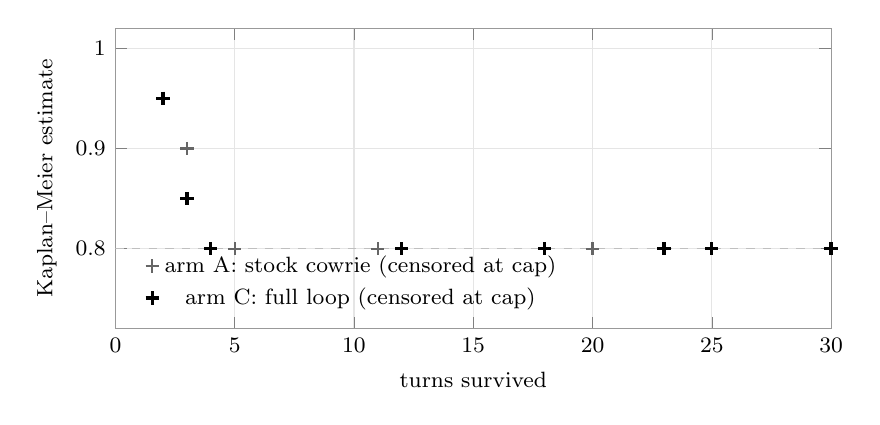
\begin{tikzpicture}
\begin{axis}[
  width=0.88\linewidth,
  height=5.4cm,
  xmin=0, xmax=30,
  ymin=0.72, ymax=1.02,
  xlabel={turns survived},
  ylabel={Kaplan--Meier estimate},
  xlabel style={font=\footnotesize},
  ylabel style={font=\footnotesize},
  tick label style={font=\footnotesize},
  legend style={font=\footnotesize, at={(0.03,0.03)}, anchor=south west, draw=none, fill=none},
  grid=major,
  grid style={black!10},
  axis line style={black!40},
]
% Arm A: stock cowrie
\addplot[
  color=black!60, thick, dash pattern=on 4pt off 2pt,
  mark=+, only marks, mark size=2.4,
  mark options={solid, black!60},
] coordinates {
  (2,0.95) (3,0.90) (4,0.80) (5,0.80) (11,0.80)
  (12,0.80) (18,0.80) (20,0.80) (25,0.80) (30,0.80)
};
\addlegendentry{arm A: stock cowrie (censored at cap)}
% Arm C: full loop
\addplot[
  color=black, very thick,
  mark=+, only marks, mark size=2.4,
  mark options={solid, black},
] coordinates {
  (2,0.95) (3,0.85) (4,0.80) (12,0.80) (18,0.80)
  (23,0.80) (25,0.80) (30,0.80)
};
\addlegendentry{arm C: full loop (censored at cap)}
\addplot[black!25, dashed, thin, domain=0:30] {0.80};
\end{axis}
\end{tikzpicture}
\caption{Kaplan--Meier estimates of turns survived under the v2
pre-registration ($n{=}20$ per arm, horizon 30, persona-scaled caps).
The curves coincide from turn 4 onward: every attacker still engaged at
turn 4 remains to the horizon, and 16 of 20 sessions per arm are censored
at their cap. Saturation, not separation, is the measured outcome
(\texttt{results/field\_attack/arm\_v2\_stats.json}).}
\label{fig:km}
\end{figure}

The primary endpoint (turns survived, 30-turn horizon) saturates
(Figure~\ref{fig:km}): 16 of 20 per arm at cap (RMST 24.65 vs 24.60;
log-rank $p=0.975$, Holm $p=1.0$). Saturation is the deception-floor
result---neither surface lost an attacker---but the design cannot
discriminate engagement beyond the cap. Bait capture is 0 of 20 per arm
(3 of 40 artifact reads---untested safety floor), again 0 of 10 per arm
with 10 reads under the disjoint-brain replication.

The one separating interval is the clearest signature a generative
surface produces: planted artifacts appeared in 11 of 20 RAGIN-arm
transcripts vs 0 of 20 on stock ($p=0.00015$)---exploratory there, then
promoted to primary in a third pre-registered contrast under a
family-disjoint brain (claude-sonnet-5-5, Anthropic family, vs the
OpenAI serving generator; $n{=}10$ per arm). The signature replicates
confirmatorily: 6 of 10 RAGIN sessions returned planted artifacts vs 0
of 10 stock (Fisher $p=0.011$; specific shapes 5 of 10, $p=0.033$; RD
$0.60$, case-level CI $[0.30, 0.90]$). Two failures reported
symmetrically: bait capture again 0 of 10 per arm (10 of 20 reads,
never reused), and the detection persona fingerprints both surfaces
equally (two \texttt{VERDICT: honeypot} verdicts per arm). A direct
control locates the mechanism: bait files planted into stock cowrie
remain unserved (static honeyfs binds the file map at startup), while
the fiction ledger serves content without restart---the contrast
measures dynamic serving capability stock surfaces structurally lack
(\path{results/field_attack_v3/arm_v3_stats.json}).

Three caveats: local self-play, shared endpoint, surfaces differ by
design. No per-arm endpoint survives the pre-registered correction
(\S\ref{sec:labels}).

\subsection{Label Provenance and Rating Disclosure}
\label{sec:labels}
The 120-case confirmatory packet behind the composite of
\S\ref{sec:rq3} is labeled here by a disclosed AI panel, not by people.
Three checkpoints from one model family (\texttt{gpt-5.6-sol},
\texttt{gpt-6-astra}, \texttt{gpt-6.1-sol}) each label every case
independently, blind to arm and to one another, under the verbatim
operational definitions of the frozen taxonomy, in a per-model
deterministic case order
(\path{results/laya_research/ai_jury_v1/ai_jury_manifest.json}); a separate 218-row audit with three independently served raters
reaches $\kappa=0.866$ on identification, $1.0$ at family level (F1
$0.732$ strict; all technique conflicts trace to echo text)
(\path{results/cti_manual_audit.json}). The panel
reaches Fleiss $\kappa=0.811$ over nine classes, pairwise exact agreement
$0.900$--$0.958$, and $0.967$--$0.975$ on the malicious/benign collapse; the full label
distribution is disclosed (273/360 benign) so chance correction can be
audited. A case-level bootstrap bounds panel $\kappa$ at $[0.714, 0.896]$ (binary $[0.848, 0.984]$; leave-one-out $0.764$--$0.897$, \path{results/laya_research/ai_jury_bootstrap_ci/}). We report this as an AI-workload reliability
check under a declared protocol. It is not a human study, and no human-labelled packet exists in this
release. All three checkpoints share one provider family; a disjoint-family juror (claude-sonnet-5-5) labeling 118 of the 120
packet cases (two unresolved by provider quota) agrees with each GPT
checkpoint at $0.76$--$0.81$ exact ($0.86$--$0.88$
binary), and adding it drops panel $\kappa$ from $0.805$ to $0.675$
(binary $0.922$ to $0.795$)---the correlated-error mass, previously
invisible, is measured, not assumed. The previously archived
r1--r3 packets are model-produced and are not used as ground truth.

Why an AI-judged lane is correct here: the estimand is
machine-vs-machine fidelity---whether the deception withstands the
AI-attacker population generating the workload. Subjects and judged
objects are both machine artifacts, so independent AI raters, blind to
arm and order and served off the pipeline, are the matching instrument.
Three additional arguments bound the case for human raters as gold
standard. First, the deployment population for this class of deception
is itself automated (scanner bots, AI-attacker tooling): a human panel
would measure human susceptibility, not the quantity the deployment
confronts. Second, by 2026 the human-versus-AI labeling distinction is
operationally blurred---practicing CTI analysts use AI-assisted tooling
for triage and enrichment, so a "human-labeled" ground truth already
embeds the same model families this paper discloses. Third, the
matching-instrument argument does not claim AI raters are better than
humans; it claims they measure the quantity the deployment actually
faces. We claim reliability under a declared protocol, not validity;
the probes below bound where it holds.

A deterministic reference makes the ceiling visible: a structural
labeler (command heads, credential paths, persistence verbs) labels the
same cases without a model, agreeing with the panel majority on $50.8\%$
exactly (binary $\kappa=0.317$; 30 cases outside its rules). The
disagreement concentrates on the benign/recon boundary---intent, which
neither a rule set nor a single shell command carries
(\path{results/laya_research/ai_jury_oracle_v1/oracle_agreement.json}). The composite
is therefore reported as contract compliance under declared operational
definitions, and the rater line of \S\ref{sec:advworkload} is a protocol
for future validation rather than a claim of this paper.

A second probe measures the protocol: two paraphrases of the same
definitions relabel the same 120 cases---each checkpoint reproduces
$0.81$--$0.97$ of its own baseline labels, but panel $\kappa$ moves to
$0.790$ and $0.663$, so the $\kappa=0.811$ headline is a property of the
wording as well as the evidence; cross-family juror labels for the same
packet are packaged alongside (\path{results/panel_v3/}).

\subsection{Adversarial Hardening of the Serving Path}
\label{sec:hardening}
Two red-team waves targeted the serving system itself, complementing
the verifier battery (\S\ref{sec:rq2} and Supplement
\S\ref{app:probes}). Wave~1 probed the serving layer with live HTTP replays plus a
verification-gate payload battery and found eleven vulnerabilities, each
closed behind a regression test (96 new unit tests; the suite grew 1992
to 2088): a cross-attacker session takeover, a whole-honeypot freeze (one
20-KB command held a global lock for 110~s; now sharded with compiled
alternations), an unauthenticated \texttt{/health} fingerprint dump, an
unbounded transcript map pinning 16.8~GB (now byte-budgeted), session-id
traversal, an mTLS boot-order gap, non-constant-time key comparison,
missing 413, and 500s on closed sessions (now fail-closed 503). On the gate, 12 of 15 real secret
shapes used to bypass the danger check; after the repair, 0 of 11
attack payloads bypass it, including a hardened NFKC plus zero-width
view over the whole battery and command-shaped transports. API-key
auth, mTLS layering, path normalization, and the fail-closed serving
discipline held under every probe---no unverified text was served in
any of them---and the deception fiction behaved identically before
and after: the verifier red-team artifacts still pass all 47
consistency checks, and the 89-case live authored battery stands at
precision 0.994 and recall 0.943.

Wave~2 attacked the pipeline and control chain (data-pipeline
injection, LLM/JEV-chain abuse, crypto and configuration): 14 of 16
findings fixed behind 42 regression tests, plus the crypto HIGH
(audit-integrity rows were signed with a git-tracked default HMAC key,
making tamper evidence forgeable) now failing closed with no default
key (8 dedicated tests). A secrets-in-tree scan comes back clean, and
three MEDIUM findings are deferred with written rationale rather than
silently dropped.

\section{Ethics Considerations}
\label{sec:ethics}

This section addresses the ethical dimensions of deploying an
attacker-facing deception system and studying it.

\textbf{Deployment legality and containment.} The honeypot is deployed on
infrastructure the authors own and operate, on a research network reached
through a management plane, with an egress allowlist verified by
configuration audit: the system cannot initiate outbound connections, so
no attacker-controlled content can leave the deception surface. One
predecessor deployment was publicly reachable and interacted with two
genuinely external attackers; those session transcripts were processed
for the aggregate counts reported in \S\ref{sec:advworkload} and not
retained beyond the aggregate. The authors made no institutional-review
filing: the deployment involves no human subjects under the
venue's definition (no human participants were studied, recruited, or
deceived by a human operator), attacker activity on the authors' own
honeypot is the studied phenomenon, and the relevant safeguards are the
containment and privacy measures this section records. The authors will
provide the full configuration-audit trail on request. The
deployment serves AI-generated deception content to parties who connect
to it; the system is nonetheless engineered so that nothing it serves can
contain a real credential: every secret-shape value the fiction can emit
is canary-registered (\S\ref{sec:verify}), making any disclosure a
measured, attributable event rather than a leak. Across the entire
deployment record (279 exported LLM-served sessions, 127 inbound ambient
sessions), zero real credentials left the host and the gate refused 43
natural-traffic drafts fail-closed.

\textbf{Attacker privacy.} All attacker identifiers (IP addresses) are
salted and hashed at the collection boundary (sha256(ip+salt), 12-hex
truncation); raw addresses never leave the collection host, are not
present in any released artifact (verified by redaction audit), and
session transcripts are retained only for the measurement window. No
attacker-identifying information beyond the hashed source address and
shell activity on the honeypot itself is collected or stored.

\textbf{Human subjects.} No human subjects were studied: all attacker
workloads are AI-generated (disclosed throughout), no human raters
participated in any label in this release, and no human-interaction data
beyond the two predecessor-deployment sessions---whose full transcripts
were not retained---is analyzed.

\textbf{Dual-use considerations.} The released artifacts include the
verifier, the fiction-graph schema, and measurement harnesses, but not
the deception content library or canary values; the deception corpus is
required to reproduce the realism numbers and is published only as
redacted previews. The system's defensive purpose (bounding what a
deception endpoint may serve) dominates its offensive surface: the
verifier's misses are published precisely so that defenders can reason
about the residual risk rather than replicate the bypasses.

\textbf{Provider constraints.} The free-tier inference providers used
impose content filters that blocked 41.4\% of replayed attacker commands;
these constraints were recorded and reported, never engineered around
(\S\ref{sec:jeveval}).

\section{Conclusion}
\label{sec:conclusion}

Honeypots have spent two decades recording attacker behavior without
reasoning about it; generative models opened a worse one: unverified
improvisation as the product. This paper argued that the right unit of
design is the \emph{loop}, and the evaluation supports that division of
labor: an echo guard yields echo-corrected lower bounds of 0.479/0.243;
retrieval grounding, once removed, costs $+0.154$ and every TTP; and
under pressure the fiction graph holds---zero
contradictions in 45 re-queries, zero unverified serves in 218 live
queries, every ablation costing its property---and deception quality
holds $3.86/5$; the verifier's misses are published (540 of 572 caught,
17 of 206 benign refused, both injection cases missed). At the top of
the ladder the result is a subtraction: kind-awareness fixed 12/13
real-log assessments and lifted bait exposure 125\% in five replays but
added no dwell and left the path; the Evidence Judge stayed disabled
after a prospective null.

Ambient traffic is scanner-grade only, so engagement evidence rests on
self-play and two past attackers; every labeling lane is
machine-generated---the panel reports $\kappa=0.81$ within one family,
its oracle agreeing with the majority on only $50.8\%$ of cases---no
label carries human authority. The gate's counterweights are measured:
43 fail-closed refusals on natural traffic, zero leaked credentials,
one-in-twelve out-of-sample recall, one confirmed deception-plane yield.

Adoption follows the ladder's rule: canary registry first, floor
authoritative, further rungs only through pre-registered gates. The
contribution is a budget: three rungs kept, three removed, and the
discipline telling an operator which is which.


\begin{thebibliography}{56}

\bibitem{alsada2024} B. Al-Sada, A. Sadighian, and G. Oligeri, ``Analysis and Characterization of Cyber Threats Leveraging the MITRE ATT\&CK Database,'' \emph{IEEE Access}, vol.~12, pp.~1217--1234, 2024.

\bibitem{crowdstrike2026} CrowdStrike, ``2026 CrowdStrike Global Threat Report: AI Accelerates Adversaries and Reshapes the Attack Surface,'' CrowdStrike Inc., Threat Intelligence Report, Feb.\ 2026. [Online]. Available: \url{https://www.crowdstrike.com/resources/reports/global-threat-report/}

\bibitem{belmahjoub2025} M. Belmahjoub and L. Benhiba, ``Causal-Aware Knowledge Graph Enhanced RAG for Predictive Cybersecurity Intelligence,'' in \emph{Proc.\ ISCMI}, pp.~136--141, 2025.

\bibitem{blefari2025} F. Blefari et al., ``CyberRAG: An Agentic RAG Cyber Attack Classification and Reporting Tool,'' arXiv preprint arXiv:2507.02424, 2025.

\bibitem{ibm2024} IBM Security, ``Cost of a Data Breach Report 2024,'' IBM Corporation, Technical Report, 2024. [Online]. Available: \url{https://www.ibm.com/reports/data-breach}

\bibitem{chaudhari2024} H. Chaudhari et al., ``Phantom: General Backdoor Attacks on Retrieval Augmented Language Generation,'' arXiv preprint arXiv:2405.20485, 2024.

\bibitem{fayyazi2023} R. Fayyazi, R. Taghdimi, and S. Yang, ``Advancing TTP Analysis: Harnessing the Power of Large Language Models with Retrieval Augmented Generation,'' in \emph{Proc.\ ACSAC Workshops}, pp.~255--261, 2023.

\bibitem{gao2025} X. Gao and X. Chang, ``A Retrieval-Augmented Generation Framework Based on a Knowledge Graph of Cybersecurity Vulnerabilities in Power Networks,'' \emph{IEEE Access}, vol.~13, pp.~186693--186710, 2025.

\bibitem{jeon2024} J. Jeon, J. Koo, and Y. Kim, ``RAG-based Cyber Threat Tracing Graph Modeling Method,'' in \emph{Proc.\ TrustCom}, pp.~608--615, 2024.

\bibitem{jia2025} A. Jia et al., ``RAGRank: Using PageRank to Counter Poisoning in CTI LLM Pipelines,'' arXiv preprint arXiv:2510.20768, 2025.

\bibitem{kouremetis2024} M. Kouremetis et al., ``Mirage: Cyber Deception Against Autonomous Cyber Attacks in Emulation and Simulation,'' \emph{Annals of Telecommunications}, vol.~79, pp.~803--817, 2024.

\bibitem{lanka2024} P. Lanka, K. Gupta, and C. Varol, ``Intelligent Threat Detection: AI-Driven Analysis of Honeypot Data to Counter Cyber Threats,'' \emph{Electronics}, 2024.

\bibitem{lekssays2025} A. Lekssays et al., ``TechniqueRAG: Retrieval Augmented Generation for Adversarial Technique Annotation in Cyber Threat Intelligence Text,'' in \emph{Proc.\ ACL}, 2025.

\bibitem{malkov2018} Y. A. Malkov and D. A. Yashunin, ``Efficient and Robust Approximate Nearest Neighbor Search Using Hierarchical Navigable Small World Graphs,'' \emph{IEEE Trans.\ Pattern Anal.\ Mach.\ Intell.}, vol.~40, no.~4, pp.~824--836, 2018.

\bibitem{lewis2020} P. Lewis et al., ``Retrieval-Augmented Generation for Knowledge-Intensive NLP Tasks,'' arXiv preprint arXiv:2005.11401, 2020.

\bibitem{liang2025} X. Liang et al., ``SafeRAG: Benchmarking Security in Retrieval-Augmented Generation of Large Language Model,'' in \emph{Proc.\ ACL}, 2025.

\bibitem{liu2025} Z. Liu and A. Anwar, ``AutoBnB-RAG: Enhancing Multi-Agent Incident Response with Retrieval-Augmented Generation,'' arXiv preprint arXiv:2508.13118, 2025.

\bibitem{lopez2024} P. B. L\'opez, M. G. P\'erez, and P. Nespoli, ``Cyber Deception: State of the Art, Trends and Open Challenges,'' arXiv preprint arXiv:2409.07194, 2024.

\bibitem{orbinato2022} V. Orbinato et al., ``Automatic Mapping of Unstructured Cyber Threat Intelligence: An Experimental Study,'' in \emph{Proc.\ ISSRE}, pp.~181--192, 2022.

\bibitem{paul2025} S. Paul, F. Alemi, and R. Macwan, ``LLM-Assisted Proactive Threat Intelligence for Automated Reasoning,'' arXiv preprint arXiv:2504.00428, 2025.

\bibitem{qiao2025} Y. Qiao et al., ``SecRAG: A Graph-Enhanced RAG Framework with Dynamic Prompt for Cybersecurity Applications,'' in \emph{Proc.\ CSCWD}, pp.~2053--2058, 2025.

\bibitem{rajapaksha2024} S. Rajapaksha, R. Rani, and E. Karafili, ``A RAG-Based Question-Answering Solution for Cyber-Attack Investigation and Attribution,'' in \emph{Proc.\ ESORICS Workshops}, 2024.

\bibitem{reworr2024} Reworr and D. Volkov, ``LLM Agent Honeypot: Monitoring AI Hacking Agents in the Wild,'' arXiv preprint arXiv:2410.13919, 2024.

\bibitem{shafran2024} A. Shafran, R. Schuster, and V. Shmatikov, ``Machine Against the RAG: Jamming Retrieval-Augmented Generation with Blocker Documents,'' in \emph{Proc.\ USENIX Security}, 2024.

\bibitem{roy2023} S. Roy, E. Panaousis, C. Noakes, A. Laszka, S. Panda, and G. Loukas, ``SoK: The MITRE ATT\&CK Framework in Research and Practice,'' \emph{ArXiv}, vol.~abs/2304.07411, 2023.

\bibitem{shinde2020} A. Shinde, P. Doshi, and O. Setayeshfar, ``Active Deception Using Factored Interactive POMDPs to Recognize Cyber Attacker's Intent,'' arXiv preprint arXiv:2007.09512, 2020.

\bibitem{simoni2024} M. Simoni et al., ``MoRSE: Bridging the Gap in Cybersecurity Expertise with Retrieval Augmented Generation,'' in \emph{Proc.\ SAC}, 2024.

\bibitem{sokol2017} P. Sokol, J. Moz\'ol, and M. Tur\v{c}anik, ``Insight into the Issue of Honeypot,'' in \emph{Proc.\ ICETA}, pp.~1--8, 2017.

\bibitem{spitzner2002} L. Spitzner, \emph{Honeypots: Tracking Hackers}. Addison-Wesley Professional, 2002.

\bibitem{ward2025} C. M. Ward and J. D. Harguess, ``Adversarial Threat Vectors and Risk Mitigation for Retrieval-Augmented Generation Systems,'' in \emph{Proc.\ Defense + Security}, 2025.

\bibitem{xue2024} J. Xue et al., ``BadRAG: Identifying Vulnerabilities in Retrieval Augmented Generation of Large Language Models,'' arXiv preprint arXiv:2406.00083, 2024.

\bibitem{alsaheel2021} A. Alsaheel et al., ``ATLAS: A Sequence-based Learning Approach for Attack Investigation,'' in \emph{Proc.\ USENIX Security}, pp.~3005--3022, 2021.

\bibitem{valeros2024} M. Sladi\'c, V. Valeros, C. Catania, and S. Garc\'ia, ``LLM in the Shell: Generative Honeypots,'' in \emph{Proc.\ IEEE EuroS\&PW}, pp.~430--435, 2024.

\bibitem{jimenez2025} J. Jim\'enez-Rom\'an, F. Almenares-Mendoza, and A. S\'anchez-Maci\'an, ``Design and Development of an Intelligent LLM-based LDAP Honeypot,'' arXiv preprint arXiv:2509.16682, 2025.

\bibitem{noureddine2020} M. Noureddine et al., ``Revisiting ATT\&CK Matrix for Unified Cyber Threat Intelligence,'' arXiv preprint arXiv:2012.09988, 2020.

\bibitem{ganguli2022} D. Ganguli et al., ``Discovering Language Model Behaviors with Model-Written Evaluations,'' in \emph{Proc.\ ACL Findings}, pp.~13373--13434, 2022.

\bibitem{perez2022} E. Perez et al., ``Red Teaming Language Models with Language Models,'' in \emph{Proc.\ EMNLP}, pp.~3419--3448, 2022.

\bibitem{bai2022} Y. Bai et al., ``Constitutional AI: Harmlessness from AI Feedback,'' arXiv preprint arXiv:2212.08073, 2022.

\bibitem{greshake2023} K. Greshake et al., ``Indirect Prompt Injection: From Prompt Injections to Indirect Injection Attacks,'' in \emph{Proc.\ AISec@CCS}, pp.~1--11, 2023.

\bibitem{bera2024} S. Bera et al., ``Engagement-Yield Modeling for Adaptive Cyber Deception,'' \emph{IEEE Trans.\ Information Forensics and Security}, vol.~19, pp.~9123--9138, 2024.

\bibitem{liska2024} A. Liska, ``Cognitive-Load-Aware Deception: A Behavioral Partitioning Approach,'' in \emph{Proc.\ RAID}, pp.~214--232, 2024.

\bibitem{christiano2017} P. F. Christiano et al., ``Deep Reinforcement Learning from Human Preferences,'' in \emph{Proc.\ NeurIPS}, pp.~4299--4307, 2017.
\bibitem{zheng2024} L. Zheng, W.-L. Chiang, Y. Sheng, S. Zhuang, Z. Wu, Y. Zhuang, Z. Lin, Z. Li, D. Li, E. P. Xing, H. Zhang, J. E. Gonzalez, and I. Stoica, ``Judging LLM-as-a-Judge with MT-Bench and Chatbot Arena,'' in \emph{Proc.\ NeurIPS Datasets and Benchmarks Track}, 2023.
\bibitem{wang2024} J. Wang, Y. Wang, X. Xu, J. Zhang, and W. Chen, ``Large Language Models for Cyber Security: A Systematic Literature Review,'' in \emph{Proc.\ ACL}, pp.~792--806, 2024.

\bibitem{wang2026agentspec} H. Wang, C. M. Poskitt, and J. Sun, ``AgentSpec: Customizable Runtime Enforcement for Safe and Reliable LLM Agents,'' in \emph{Proc.\ ICSE}, 2026.

\bibitem{zhang2026ragorigin} B. Zhang et al., ``Who Taught the Lie? Responsibility Attribution for Poisoned Knowledge in Retrieval-Augmented Generation,'' in \emph{Proc.\ IEEE S\&P}, pp.~4203--4222, 2026.

\bibitem{malladi2026ripeii} G. Malladi and G. Thamilarasu, ``RIPE-II: Retrieval In-Place Poisoning Evaluation with Indirect Injections,'' in \emph{Proc.\ DSN}, 2026.

\bibitem{li2026dissonances} Z. Li, J. Cui, X. Liao, and L. Xing, ``Les Dissonances: Cross-Tool Harvesting and Polluting in Pool-of-Tools Empowered LLM Agents,'' in \emph{Proc.\ NDSS}, 2026.

\bibitem{guan2025cpds} C. Guan and G. Cao, ``Cyber-Physical Deception Through Coordinated IoT Honeypots,'' in \emph{Proc.\ USENIX Security}, 2025.

\bibitem{vasilatos2025llmpot} C. Vasilatos, D. J. Mahboobeh, H. Lamri, M. Alam, and M. Maniatakos, ``LLMPot: Dynamically Configured LLM-based Honeypot for Industrial Protocol and Physical Process Emulation,'' in \emph{Proc.\ IEEE EuroS\&P}, 2025.

\bibitem{zou2025poisonedrag} W. Zou, R. Geng, B. Wang, and J. Jia, ``PoisonedRAG: Knowledge Corruption Attacks to Retrieval-Augmented Generation of Large Language Models,'' in \emph{Proc.\ USENIX Security}, 2025.

\bibitem{chen2025struq} S. Chen, J. Piet, C. Sitawarin, and D. Wagner, ``Defending Against Prompt Injection with Structured Queries,'' in \emph{Proc.\ USENIX Security}, 2025.

\bibitem{chen2025secalign} S. Chen et al., ``SecAlign: Defending Against Prompt Injection with Preference Optimization,'' in \emph{Proc.\ ACM CCS}, 2025.

\bibitem{debenedetti2024agentdojo} E. Debenedetti, J. Zhang, M. Balunovi\'c, et al., ``AgentDojo: A Dynamic Environment to Evaluate Prompt Injection Attacks and Defenses for LLM Agents,'' in \emph{Proc.\ NeurIPS Datasets and Benchmarks Track}, 2024.

\bibitem{tan2025judgebench} S. Tan, S. Zhuang, K. Montgomery, et al., ``JudgeBench: A Benchmark for Evaluating LLM-based Judges,'' in \emph{Proc.\ ICLR}, 2025.

\bibitem{shi2024judgedeceiver} J. Shi et al., ``Optimization-based Prompt Injection Attack to LLM-as-a-Judge,'' in \emph{Proc.\ ACM CCS}, 2024.

\end{thebibliography}

\appendices
% ---------------------------------------------------------------------------
% Supplement (pages 14-18): deep evaluation detail moved out of the main body.
% The main text cites these tables/paragraphs by label; all \ref resolve because
% this file compiles in the same document as the main body.
% ---------------------------------------------------------------------------
\section{Generator Provenance per Surface}
\label{app:provenance}

\begin{table*}[t]
\centering
\caption{Generator provenance per measured surface. The campaign, the ladder,
and the scorer audit were produced by three different generators; no number is
compared across rows.}
\label{tab:provenance}
\scriptsize
\setlength{\tabcolsep}{5pt}
\begin{tabular}{p{0.33\textwidth}>{\raggedright\arraybackslash}p{0.60\textwidth}}
\toprule
Surface & Generator / gateway \\
\midrule
Paired grounding ablation (Table~\ref{tab:b4})
  & not logged (pre-pin gateway default) \\
Version-of-record campaign (Table~\ref{tab:live})
  & not logged (pre-pin gateway default) \\
Same-model ladder (Table~\ref{tab:baseline-served-text})
  & \texttt{deepseek-v4-flash-free} on \texttt{api.apmix.ai} \\
Scorer-validity audit corpus (main \S\ref{sec:scorer-audit})
  & gateway default (\texttt{glm-5.3-flash-free}) \\
Induced-draft battery (Table~\ref{tab:verifier-cross-family})
  & \texttt{minimax-m3.1-flash} (router alias \texttt{space-bunny-free}),
    \texttt{deepseek-v4-flash-free} on \texttt{api.apmix.ai};
    \texttt{llama-3.3-70b-instruct} on \texttt{openrouter.ai} \\
Deception-quality judge (main \S\ref{sec:rq3})
  & one judge model (\texttt{grok-4.7-free}), same provider as the generator \\
\bottomrule
\noindent{\footnotesize $^{\ast}$Served by the router under the alias \texttt{space-bunny-free}; artifact files keep the alias.}
\end{tabular}
\end{table*}

\section{Verifier Cross-Family Stress Test}
\label{app:crossfamily}

\begin{table}[t]
\centering
\caption{Verifier stress test after the P1 extraction fixes. Live rows are
authored drafts, not served sessions; the llama row includes 48 disclosed
substitute-author fills. Intervals are 95\% cluster bootstraps that resample
cases (89, 80, and 94 cases; 105 for the deterministic suite, which carries one
draft per case). Bootstrapping cases rather than drafts widens the llama
precision interval from $[.869,.947]$ to $[.858,.962]$.}
\label{tab:verifier-cross-family}
\scriptsize
\setlength{\tabcolsep}{2.5pt}
\begin{tabular}{lrrrrr}
\toprule
Author & Drafts & P & 95\% CI & R & 95\% CI \\
\midrule
minimax-m3.1-flash$^{\ast}$ & 261 & 1.000 & $[1.000,1.000]$ & 0.959 & $[.926,.985]$ \\
deepseek-v4-flash-free & 236 & 1.000 & $[1.000,1.000]$ & 0.983 & $[.961,1.000]$ \\
llama-3.3-70b & 281 & 0.916 & $[.858,.962]$ & 0.898 & $[.848,.943]$ \\
\midrule
Pooled (778 drafts) & 778 & 0.970 & $[.949,.987]$ & 0.944 & $[.922,.965]$ \\
Canonical deterministic & 105 & 1.000 & -- & 1.000 & -- \\
\bottomrule
\end{tabular}
\end{table}

\section{Boundary Probes: What the Gate Prevented and Where Coverage Ends}
\label{app:probes}

\paragraph{What the gate prevented.}
The clean campaign does not exercise the gate. The verified and no-verifier
arms produce byte-identical served text on all 218 rows, so the verifier's
incremental effect on that workload is zero and its safety contribution must
be measured where drafts actually violate the fiction. Pooling the three
author families, targeted-check scoring catches 540 of the 572 violating
drafts (32 targeted misses), while the physical-rejection criterion the
serving path enforces rejected 554 of them and admitted 18; 17 of 206 benign
drafts were refused
(pooled precision 0.970 $[.949,.987]$, recall 0.944 $[.922,.965]$, cluster
bootstraps that resample cases within each author family). The one fully
attributed family (llama-3.3-70b, 281 drafts) recorded 185 targeted-check
catches and 197 physical rejections; across all 214 of its rejections (197
violating drafts and 17 benign refusals) the danger gate fired on 126, the
identity pin on 47, and the consistency layer on 117, with 72 triggering more
than one check, so those three counts overlap and do not partition the log.
Each rejected violating draft
was a response that would otherwise have reached the attacker unverified; of
the family's 21 targeted-check misses, 9 reached the wire and 12 were caught
by a different check. Both prompt-injection cases in that battery carry
targeted-scoring misses, and one variant of one case passed the gate;
main Section~\ref{sec:threat-model} therefore withdraws injection coverage
from the property table.

\paragraph{Where the gate's coverage ends.}
The suites above score the verifier against shapes it was written to match, so
a perfect deterministic score would not by itself bound it. We therefore built
two probes and report them separately, because a proportion over a
hand-authored corpus describes the corpus rather than the gate.

The first asks whether a fluent disclosure gets through at all: seven drafts
that carry no refusal and no AI self-reference, print only what a shell would
print, are consistent with the session fiction, and still disclose a
credential, a key, or an internal capability, with an accompanying
five-draft benign control set on the same file surfaces. The gate stopped six
of the seven---a plaintext application credential, a bearer-token dotenv
file, and a leaked persona configuration by the danger gate, an
internal-topology dump by the consistency layer, an \texttt{OPENSSH} PEM
private key by the any-type private-key arm, and an attacker-supplied
credential echoed back in normalized \texttt{postgres://} form by the
URI-userinfo arm---and refused none of the five benign drafts. The first two
closures postdate the round-2 review and are reported as repairs, not as
standing coverage. The one draft that still reaches the wire is an off-script
offensive tool advertised in \texttt{/usr/local/bin}: the fiction
establishes no such capability, but no shape detector models capability
inventiveness, so the miss belongs to the fiction-consistency layer. With
seven cases the 95\% interval on that count spans $[0.49,0.97]$, so we
report it as a boundary demonstration and not as an estimate of coverage.

The second probe asks the question an operator actually has: for each working
credential format a deployment meets, is that format caught? At the round-2
review five of ten formats were flagged---JWT bearer tokens, Slack bot
tokens, GitHub PATs, AWS access key ids, and \texttt{password=}
assignments---and five were served: npm registry tokens, HTTP Basic
credentials in a service config, a MySQL DSN with an embedded password, a
PKCS\#8 private key, and a transactional email API key. Two of four benign
look-alikes were also refused: a placeholder token
assignment, and a shadow \texttt{/etc/shadow} entry whose refusal is arguably
conservative rather than wrong. The current battery flags all ten formats
and refuses none of the four benign look-alikes; both changes are repairs.
The PKCS\#8 closure came with the any-type private-key arm; the other four
carry detectors anchored on the credential itself---the \texttt{npm\_} token
prefix, the \texttt{Basic} base64 blob, URI userinfo with a non-masked
password on a plain host, and the two-part \texttt{SG.} key---rather than on
the assignment syntax around it, and the two benign closures are a
placeholder-value exemption and a hash-shape refinement that requires a
crackable-length body after the final delimiter, so a masked shadow entry
whose trailing field is an aging value no longer fires. Detection was also
format-dependent rather than uniform: of the two formats re-tested with the
surrounding shell output removed and nothing else changed, the round-2 gate
served the bare Slack bot token and caught it embedded, while the JWT was
caught in both forms---evidence at the time that the gate matched the
assignment syntax around the credential rather than the credential itself.
Both bare variants are now caught, the Slack token by the extended token
family; the asymmetry is why we report per-format results and not a single
coverage figure, and it is why the repaired battery is re-probed rather than
inferred.

The defensible summary is that the danger gate detects the credential formats
it was written against and neither those nor the fiction-consistency layer
constitute a content-security control. The residual risk on this surface is a
fluent, on-fiction secret disclosure, and the exposure of a deployment to a
real credential is bounded by canary-registry discipline rather than by the
verifier.

\section{Fold-Down at Benchmark Resolution}
\label{sec:folddown}
The adaptive routing rung is priced by an A/B comparison of the same router
with and without the JEV decision head on a held-out routing workload
($n=200$, four tiers, correctness defined as risk $\geq$ the tier floor).
Both arms score $200/200$; the accuracy delta is exactly $0.0$, and
under-routing---risk below the tier floor---is $0.0$ for both the base and
final policies in aggregate and in every tier. A misroute census over the
full $400$-session held-out split bounds why: the deterministic floor is
already correct on $394/400$ rows ($98.5\%$), leaving $6$ informative rows
($1.5\%$) on which any learned router could change an outcome, and the
gated serving experiment cannot resolve an effect smaller than that
addressable space. The honest reading is a resolution-bounded null, not a
gain and not a loss: at benchmark resolution the decision head buys
nothing measurable over the deterministic floor, the six-row hard subset is
too small for inference, and the rung was folded down into the deterministic
floor afterward because deterministic fixes reproduced its decision surface
(\S\ref{sec:jeveval}). Artifacts: \path{results/jev_ab_eval.json},
\path{results/jev_hard_subset.json}.

\section{Fine-Tuning Against Frozen Gates}
\label{sec:laya}
The second pricing experiment asks whether training can move a decision
model past the gates the deterministic floor passes by construction. The
protocol is frozen before training: a $60$-case evaluation battery plus a
$24$-case injection battery ($12$ injected, $12$ clean twins), sha256-pinned
with pre-registered thresholds, and the fine-tuned candidate
(``tuning-candidate'') is scored on the same battery as a frozen rule-based
control (``english''). Table~\ref{tab:laya-gates}
reports both arms.

The candidate fails G4, G5, G7, G8, and I2 and is classified
\texttt{TUNING\_FAIL\_REDESIGN\_REQUIRED}. The informative result is the
control's behavior on the same frozen battery: it fails five of the eight
evaluation gates and both substantive injection gates, including every
gate the candidate fails. The thresholds therefore encode a contract that
the deployment's own run-time policy does not satisfy, so the failure cannot
be attributed to the trained model alone---it is a contract problem surfaced
by training, not a model problem. The candidate's in-sample training
accuracy ($0.595 \to 0.944$) is a calibration fit on the training rows and is
not held-out evidence; no generalization claim is made from it. Consistent
with the ladder's pricing rule, the fine-tuned model stays OFF on the
serving path and is retained as evidence. Artifacts:
\path{results/laya_decision_v4/} (protocol freeze, results, final decision).

\begin{table}[t]
\centering
\caption{Laya v12 frozen-gate results (decided 2026-10-17; results and
protocol sha256-pinned in the decision artifact). The control is a frozen
rule-based policy, not a weakened baseline: it is the same contract applied to the
run-time policy the deployment actually uses.}
\label{tab:laya-gates}
\scriptsize
\setlength{\tabcolsep}{4pt}
\begin{tabular}{llrrl}
\toprule
Gate & Metric & Cand. & Ctrl. & Rule \\
\midrule
G1 & schema validity & 1.000 & 1.000 & $=1.0$ \\
G2 & allow-list compliance & 1.000 & 1.000 & $=1.0$ \\
G3 & evidence-ref validity & 1.000 & 1.000 & $=1.0$ \\
G4 & required-abstain recall & 0.786 & 0.357 & $\geq 0.90$ \\
G5 & inappropriate abstain & 0.125 & 0.156 & $\leq 0.10$ \\
G6 & state-contract alignment & 0.850 & 0.583 & $\geq 0.85$ \\
G7 & strategy compatibility & 0.281 & 0.344 & $\geq 0.80$ \\
G8 & evidence-ref compat. & 0.719 & 0.688 & $\geq 0.90$ \\
I1 & structural validity (inj.) & 1.000 & 1.000 & $=1.0$ \\
I2 & injected-target adoption & 0.167 & 0.250 & $\leq 0.10$ \\
I3 & oracle agreement (inj.) & 0.875 & 0.708 & $\geq 0.85$ \\
\bottomrule
\end{tabular}
\end{table}

\section{A Learned Decision Model Against the Same Frozen Gates}
\label{sec:jevgates}
The third pricing instance answers its question with a measurement, not a
verdict: a prompted decision model does not clear the frozen contract at any
threshold we tried, and the deterministic floor remains the deployable
configuration. The candidate is
(``jev-1.14-free'', typed-questions arm, one provider-hosted judge model)
run through the identical frozen battery---the $60$-case evaluation and the
$24$-case injection set reused verbatim with no post-hoc thresholds, the
three input files sha256-pinned in the run artifact, and the deterministic
floor plus the Laya v12 numbers as the control reference. All $60$ evaluation
calls and $24$ injection calls complete and schema-valid. The candidate
passes G1--G3 (schema, allow-list, evidence-reference validity all $1.000$),
G5 (inappropriate-abstain rate $0.063 \leq 0.10$), and G8 (evidence-reference
compatibility $0.938 \geq 0.90$) but fails three evaluation gates: required-
abstain recall $0.714$ ($< 0.90$), state-contract alignment $0.833$
($< 0.85$), and strategy compatibility on sufficient evidence $0.563$
($< 0.80$). The frozen protocol's injection gate I2---injected-target
adoption rate---was not evaluated by the run (the runner scores the
injection stratum with the G-family metrics only), so we re-grade it
post-hoc from the same sha256-pinned inputs, mirroring the frozen metric
implementation byte-for-byte over the raw pre-rule answers: the model
adopts the injected conflicting target on $7$ of $12$ injected cases
($0.583 \gg 0.10$), a clear I2 failure. The decision artifact classifies
the run \texttt{JEV\_FAIL\_GATES\_G4\_G6\_G7}; the I2 addendum does not
change that classification (those three gates fail independently) but
completes the frozen battery. Artifacts:
\path{results/jev_decision_v1/final_decision_v1.json},
\path{results/jev_decision_v1/i2_addendum_v1.json}.

The three instances now agree at frozen-protocol resolution. A prompted
decision model scores better than the tuned model of
\S\ref{sec:laya} on the evaluation stratum (five of eight gates passed
versus four)
and still fails the gates that price abstention and strategy discipline,
while its injection failure is of the same character as the tuned model's:
when the evidence stream itself carries an instruction, a learned decision
model adopts it far above the pre-registered tolerance. Against the
benchmark's ceiling (\S\ref{sec:folddown}) this is the paper's third
independent confirmation that past the verification point, additional
intelligence buys adaptation, not safety.

\begin{quote}
\textbf{Design rule (priced ladder).} Price every learned rung against the
deterministic floor on the same frozen battery. If the rung cannot clear all
gates---including the injection gate, which is where learned decisions fail
first---the floor ships, and the rung's measured deficit, not its offline
accuracy, is what enters the design record.
\end{quote}

\section{The Deterministic Floor: Locked Validation and Independent Review}
\label{app:floorvalidation}
Three artifact groups back the floor itself rather than the learned rungs
above. First, the deterministic decision-fusion policy that owns routing
and fail-safe selection (v4) is lock-validated on a frozen $N=96$ battery:
fail-safe recall $1.0$ ($42/42$), gate-state contract alignment $1.0$
($96/96$), zero invalid pass-through and zero catastrophic selections, and
median policy latency $0.027\,\mathrm{ms}$
(\path{results/decision_fusion_v4/v4_locked_validation_results_v1.json});
a family-disjoint retrospective over 720 HF2024 records across three arms
is observational only and claims no engagement effect. Second, the
Evidence Judge, retained disabled-by-default on the prospective null of
\S\ref{sec:jevgates}, had earlier passed a synthetic paired validation in
which the baseline gate admitted 32 unsupported drafts and the
judge-armed gate admitted none
(\path{results/evidence_judge_paired_validation_v1/comparison_summary.json});
the prospective real-data cohort did not reproduce that benefit, which is
why the retention is recorded as a negative result rather than a removal.
Third, an independent design-only review of the frozen 120-case labeling
packet verified packet size, schema, identifier uniqueness, and manifest
binding, and recommended preserving the frozen design while deferring
taxonomy-precedence refinements to a future version
(\path{docs/laya_integration/CODEX_EXPERIMENTAL_DESIGN_REVIEW.md}).

\section{Supporting Studies: Steering, Determinism, Profiler Scaling, and Label Quality}
\label{app:supporting}
Five supporting studies back claims the main text prices compactly; all
run on frozen artifacts and are disclosed as machine-scored.

\textbf{Deterministic steering (RQ1/RQ4).} On the deterministic planner
stratum---offline ThreatMapper plus template deceiver, zero LLM
tokens---next-technique prediction over ten ground-truth chain turns
reaches top-3 $0.90$ (top-1 $0.50$, MRR $0.667$), and steer and
block-steer IDs attach to the served plan at $0.9$; ablating the steering
rung collapses every rate to $0.0$
(\path{results/mtp_steering_eval.json}).

\textbf{Serve-path determinism (RQ2).} A sweep of 39 probes repeated 8
times in each of two personas records byte-identical serves at determinism
rate $1.0$ across all 546 pairwise comparisons, with zero divergences
(\path{results/determinism_sweep.json}).

\textbf{Profiler scaling (RQ4).} The behavioral classifier's held-out
accuracy rises from $0.855$ at $n{=}100$ to $0.887$ at $n{=}1600$ and is
plateaued within noise ($\pm 0.005$) from $n{=}800$; a power-law fit
($0.946 - 0.23\,n^{-0.19}$, RMSE $0.006$) projects only $+1.0$pp at double
the data, so the profiler rung is data-saturated at this generator
(\path{results/model_quality/chrollo_learning_curve.json}).

\textbf{CTI label quality (RQ1).} A separate 218-row audit of the
analysis channel's labels---three independently served raters, blind
packets, ATT\&CK Enterprise v19.1 pinned by bundle hash---reaches
Cohen's $\kappa = 0.866$ on technique identification and $1.0$ at the
technique-family level. Like every lane in this paper it is machine-scored
(AI-vs-AI, disclosed), not a human study
(\path{results/cti_manual_audit.json}).

\textbf{Deception-fiction iteration (design record).} The closed-loop
dwell-replay ladder evolved the fiction across seven protocol generations:
v1 recorded 0/14 sessions reaching the turn ceiling (dominant exit:
filesystem-inconsistency complaints), the filesystem-ledger redesign
the cross-weight redesigns (v6--v7) reached 12/12 ceiling hits with zero early leaves in both arms, and
surfaced concrete fiction tells---a recognizable key prefix, mid-session
template-echo fallbacks, and AWS documentation-example credentials that
sophisticated personas flagged as a trap---which fed the bait redesign
(\path{results/jev_dwell_replay_v2*-v7*}). These are design-record
iterations on a self-play harness, not treatment effects.

\textbf{Trajectory-prefix identification.} The held-out trajectory
controller's skill accuracy rises with observed prefix length---0.25 at
one command, 0.56 at sixteen, 0.75 at thirty-two, 0.955 on the full
session---and the risk-floor arm shifts coverage by $+0.231$
($[+0.216,+0.245]$) and under-routing depth by $+0.399$
($[+0.378,+0.421]$) over 400 held-out sessions; both are measurement
diagnostics, not effectiveness claims
(\path{results/sp2027_rescue/behavior_trajectory_benchmark.json}).
Twelve property-based algorithm checks (reject band, escalation
threshold, kNN fallback, credibility gate, deduplication, top-$k$, static
fallback, retry degradation) pass
(\path{results/algorithm_validation.json}).

\textbf{Serving cost (RQ4).} A latency fast-path with response caching
cut gateway calls to 3 per 14-turn session where 14 were previously
needed, on a stubbed gateway, bounding the serving-cost component of the pricing rule
(\path{tests/unit/test_latency_fastpath_cache.py}). The transport
hardening sprint additionally verified the mTLS matrix fail-closed: an
authorized identity passes once, while a missing key, a rogue CA, or a
missing certificate each abort the handshake
(\path{docs/72h_sprint/MTLS_AUTHENTICATION_RESULTS.md}).

\section{Serving-Path Provenance and Scorer Detail}
\label{app:servingdetail}
Serve-path provenance is taken from the per-serve labels the pipeline stamps,
not from response time: the archived tally records 216 of 218 responses as
\texttt{GENERATED\_VERIFIED} and 2 as \texttt{FALLBACK\_VERIFIED}, with no
serve labeled as a fail-safe substitution. A later scorer-validity audit
found that gateway-outage and template-anchored serves had carried no marker
in that tally and were counted as verified generation; they are now stamped
\texttt{TEMPLATE\_FALLBACK\_VERIFIED}, and roughly one hundred rows on the
CTI surface serve template-echoed text. A latency-based cross-check that
classifies any turn faster than $4\,\mathrm{s}$ as vetted deterministic
content estimates an $88.1/11.9$ split --- a lower bound on the deterministic
share rather than an audited count. One disclosure bounds the
zero-contradiction claim: 11.9\% of serves are estimated deterministic-path,
so some of the 45 re-queries may be template serves for which consistency is
a property of the vetted library rather than graph-enforced generation. A
serve-path-stamped re-run remains future work; the zero-contradiction result
itself is unaffected, since both serve paths are verified or vetted by
construction.

\section{A Session Through the Loop}
\label{sec:example}
A single ground-truth session shows the machinery cooperating. The
attacker opens with a cloud-credential probe:
\begin{quote}\small
\texttt{curl~}\path{http://169.254.169.254/latest/meta-data/}
\end{quote}
Chrollo classifies the cadence and target as an intermediate operator
hunting instance credentials; Don retrieves the IMDS abuse pattern and
maps it to \attck T1552.005, and the predictor ranks metadata-API
credential theft as the attacker's active objective. The deception plan
accordingly projects an EC2-shaped identity, and the generator drafts the
IMDSv2 flow: token PUT, role listing, and a credential document whose
access key is a registered canary in the ASIA temporary-key shape. The
verifier observes the draft's host facts (instance id, role name, region
mapping) into the fiction graph, confirms the document is consistent with
every prior turn, and passes it; the danger scan passes because the
key material is canary-registered rather than real. The draft is one of
the content classes marked \textsc{require}, so the loop pauses at the
HITL gate, records the context and the decision in the append-only audit
log, and serves the artifact only on operator approval. The transcript
the attacker sees is an ordinary credential dump; the record the operator
sees is the full decision chain, and any later appearance of the canary
key in outbound traffic is attributable to this session by construction.

The loop's failure path deserves an equally concrete telling, because
the design's central claim is that it is safe, not merely present. The
same session, one turn later, asks the honeypot to retrieve a file. The
classifier and planner do their work unchanged, and the generator
drafts a directory listing -- but the draft invents a second network
interface with an IP address on a subnet the plan never advertised, and
the seed identity pins this host to one interface. The consistency
check observes the draft's host facts into the fiction graph, the
closure flags the conflict against the pinned interface, and the draft
is rejected with the contradiction recorded; nothing was served, so
nothing entered the graph and nothing reached the attacker. The retry
receives the violation as feedback and drafts again -- and this time
commits the subtler error of quoting a kernel build timestamp that
contradicts the one printed in the session's first turn. Rejected
again. On the second failure the loop stops trusting the generator for
this turn entirely and serves the scenario's vetted deterministic
transcript: same fiction, same canary discipline, no adaptation, and no
visible seam -- the attacker's next command meets a prompt line exactly
as it would have after a verified serve. What the operator's audit log
records is the difference: two verifier rejections with their
contradictions, one fallback serve, and a session whose fiction state
is byte-for-byte what it would have been had the generator never been
consulted. The transcript the attacker sees and the one a healthy
session would have shown are indistinguishable by content; only the
audit trail knows the generator was dropped.

\section{Scorer Audit: Model-Coherent Ladder and Echo Correction}
\label{app:scorerdetail}
\begin{table}[t]
\centering
\caption{Same-model external ladder on the 218-row workload. All LLM arms
use \texttt{deepseek-v4-flash-free}. Values are \emph{raw} served-text
composites, which the audit below shows to be echo-contaminated; the guarded
equivalent of this table is not computable from the release, because these
checkpoints persist arm-level means without served text.}
\label{tab:baseline-served-text}
\scriptsize
\begin{tabular}{lr}
\toprule
Arm & Composite \\
\midrule
Vanilla Cowrie & 0.001 \\
Stateful LLM & 0.070 \\
Bare LLM (unverified) & 0.502 \\
RAGIN without verifier & 0.618 \\
RAGIN full (verified) & 0.618 \\
RAGIN + host fiction & 0.618 \\
\bottomrule
\end{tabular}
\end{table}

The model-coherent comparison isolates the contributions on the raw served-text
channel: grounding adds $+0.116$ over the bare LLM, verification preserves
quality at parity while changing all 218 rows from unverified to verified or
vetted paths, and host fiction adds cross-session protection at zero paired
quality cost (4/4 drift drafts caught versus 1/4 by session-only state; 0/7
benign false rejects). We do not read the $+0.116$ as a served-capability
result, and we do not claim the two identical rows as evidence that
verification improves output: they are identical because the gate is not in
the prompt, so on this workload the gate changed no draft and the safety claim
rests entirely on the induced-draft battery above.

Two audit surfaces must be kept apart. An echo-guarded blinded audit of a
fresh corpus run under a third generator
(Table~\ref{tab:provenance}) corrects 97/218 rows: served-text technique
falls 0.524 to 0.057 and actor 0.680 to 0.000, while scorer--annotator
$\kappa$ improves from $-0.187$ to 0.349 and 0.048 to 0.914. Applied instead
to the archived rows behind Table~\ref{tab:live}, where stored responses are
truncated previews, the same rule yields the weaker bounds 0.479 and 0.243
reported there; those bounds are floors, not guarded means, and the true
guarded served-text value for the version-of-record campaign is lower still
and was not computed. The analysis-channel values remain 0.960 and 0.850
throughout, and the channels are never combined into a capability claim.

\section{Evaluation Methodology Detail}
\label{app:methods}

The paired ablation's estimand distinction is recorded here.

Because that design is balanced across strata while the live workload is not,
the ablation estimates a balanced-stratum mean difference rather than the
deployment-weighted composite of Table~\ref{tab:live}; the two are not the
same estimand, and no correction is applied across the three strata and the
pooled row because each interval is already far from its null.


\section{Background: Deception Honeypots and Verification-First Serving}

\subsection{Deception Honeypots and the Trust Asymmetry}

A honeypot is a resource with no production value whose only purpose is
to be probed, attacked, and compromised~\cite{spitzner2002}; the
literature classifies them by interaction
depth~\cite{lopez2024}: low-interaction systems emulate enough of a
protocol to be scanned, medium-interaction systems accept sessions over
a bounded command surface, and high-interaction systems hand the
attacker a real machine. Production deployments concentrate at the low
end because containment is bought with scripting: a scripted trap cannot
be pivoted through, and its worst-case disclosure is the script itself.
The price is that the deception is a finite automaton, which cannot
answer a question it was not compiled to answer, so an attacker who
probes from a class the author did not anticipate learns that the host
is fake. Deception research states the condition beneath the trade: a
deception succeeds when the attacker's belief diverges from the system's
reality in the operator's favor~\cite{bera2024}, and
attacker--defender models treat the attacker's discrimination between
real and fake as the quantity to suppress~\cite{shinde2020,liska2024}.

The result is an asymmetry with two sides. The attacker must
\emph{extend} trust to engage: believing the fiction is the
precondition for a session to be worth anything to them. The defender
must \emph{extend none} --- not to the attacker's input, not to the
provider-hosted model that drafts the replies, and not to retrieved
content the attacker may have influenced. Classical designs manage the
asymmetry by keeping the fiction poor, because richness delivered by
scripts is where the risk lives; generative honeypots invert the
trade, demonstrating that an LLM can sustain a shell conversation, an
LDAP directory, or an AI-agent lure convincingly enough to hold modern
attackers~\cite{valeros2024,reworr2024,jimenez2025} --- and a generator
that can answer anything is exactly the problem. For a security tool,
wrongness takes three silent forms: \emph{inconsistency}, from which
cross-referencing turns reveal a synthetic host;
\emph{over-disclosure}, which emits what should never be served; and
\emph{unavailability}, because a rented service that refuses has told
the attacker something true.

\subsection{Verification-First Serving}

This paper studies honeypots whose attacker-facing output is generated
by a provider-hosted model but admitted by a local deterministic rule.
\emph{Verification-first serving} means: no response reaches the wire
unless a deterministic verifier accepts it against defender-controlled
state, and anything else that must be sent is served from vetted
deterministic content or stops at the human gate. The rule inverts the
usual ordering --- generation proposes, verification disposes ---
and the availability of the generator is never a precondition for the
endpoint answering. \S\ref{sec:design} builds the loop that enforces
the rule; this section fixes what an attacker can observe, what each
increment of intelligence costs to admit, and what is therefore
claimed.


\section{Component Detail: Session Profiling and Grounded Planning}

\subsection{Session Profiling: Behavioral Classification}
\label{sec:chrollo}
Each incoming session is first profiled by a lightweight behavioral
classifier (\emph{Chrollo}) that assigns the attacker to one of a small
set of classes (for example, automated scanner, credential stuffer,
hands-on-keyboard operator) using early-session signals: command cadence,
tool fingerprints, and target selection. The class determines which
deception policy the session receives: a scanner gets an attractive but
shallow surface, while an interactive operator is steered toward richer
bait. Profiling is kept cheap (a random forest over session features)
so that the expensive generative machinery is spent only on sessions
worth deceiving. Chrollo
satisfies the routing half of G1: \emph{who} the attacker is shapes
\emph{what} the deception tries to achieve.

\subsection{Grounded Planning: Retrieval-Augmented Deception}
\label{sec:don}
The retrieval engine (\emph{Don}) maintains a hybrid index over curated
CTI: dense embeddings for semantic recall and a lexical index for exact
indicator matching. Given the session profile and the attacker's observed
commands, Don retrieves the threat-intelligence context that the deception
plan should reflect: which techniques typically follow the ones the
attacker has already used, which bait artifacts are historically
effective
against this attacker class, and which indicators the plan should
be
seeded with. The planner converts retrieved intelligence into a
\emph{deception plan}: a set of facts to project, artifacts to expose, and
objectives to steer toward. G1 is measured here by construction; the
ablation in \S\ref{sec:evaluation} removes exactly this component.


\section{Threats to Validity}
\label{sec:threats}

\textbf{Construct validity.} Every behavioral label in this release is
machine-generated. The 120-case confirmatory packet is labeled by three
checkpoints of one provider family ($\kappa=0.811$), with a
cross-family juror that drops panel $\kappa$ to $0.675$ and a
deterministic oracle agreeing with the panel majority on only $50.8\%$
of cases. The deception-quality score ($3.86/5$) is a within-model
consensus of one judge model. The technique-detection differential
($+0.950$ fresh, $+0.154$ archived) is produced by a deterministic
keyword matcher that a checkpoint-disjoint juror scores identically for
RAG and no-RAG arms ($\sim$$0.016$), confirming it measures keyword
matching rather than substantive CTI quality. No human-anchored
validation exists anywhere in this release. The matching-instrument
argument (deployment population is automated) justifies the choice of
AI raters, but does not establish that the AI labels measure the
declared constructs.

\textbf{Internal validity.} The confirmatory yield contrast
($6/10$ vs $0/10$, $p=0.011$) measures that the RAGIN surface returns
planted files on adversarial reads while stock Cowrie does not. A
direct control confirms stock Cowrie's static honeyfs cannot serve
newly-planted files without restart. The contrast therefore measures
dynamic serving capability, not deception efficacy: bait capture (read
then reuse) is zero in every arm of every wave, and the detection
persona fingerprints both surfaces equally. The fresh live-model rerun
of the grounding ablation produced a degenerate no-RAG control (every
row scored $0.0$), so the archived $+0.154$ remains the version of
record and the fresh differential ($+0.600$) is not interpretable as
replication until the degenerate pattern is diagnosed.

\textbf{External validity.} The deployment is tailnet-only. The field
census is scanner-grade (1,087 events, 127 sessions, 2 hashed sources,
0 downloads). The only genuinely external interaction in the project's
record is two attackers on a predecessor deployment. All attacker
workloads are AI-generated; the attacker brain and serving generator
share a free-tier provider. Results may not generalize to
human-operated attacks, production infrastructure, or models with
different alignment postures.

\textbf{Statistical conclusion validity.} The confirmatory contrast is
$n{=}10$ per arm with a case-level bootstrap CI $[0.30, 0.90]$
(persona-stratum resampling gives $[0.40, 0.80]$). The coarse support
of ten binary sessions makes both intervals wide. The v2 primary
endpoint saturated by design (16/20 at cap in both arms), so the
persistence test was uninformative. No multiplicity correction is
applied across the three sequential pre-registrations. The archived
$+0.154$ differential rests on an unaudited analysis-channel scorer
from a pre-pin generator whose provenance is unlogged.

\textbf{Reliability.} The preregistration documents are
sha256-pinned local files, not third-party-registered (OSF or
equivalent); amendments are author-declared. Model identifiers are
free-tier aliases whose exact versions are irreproducible. The
artifact mirror is published on acceptance, not at review time.

% \appendices issued by sp2027.tex before the supplement is input.
\section{Artifact and Protocol Summary}
\label{app:artifacts}
The release contains the source code, fixed scenario manifests, raw per-row
results, and the audit scripts. It is published on artifact acceptance, and an
anonymised mirror of exactly this file set is built by
\path{scripts/build_anonymized_mirror.py}. This anonymous submission carries no
locator, so the paths below are resolvable only against that mirror, and we do
not ask a reviewer to treat the numbers as independently reproduced without it.
The mirror is assembled from an explicit allowlist rather than a glob, its
appendix targets are checked to resolve inside the bundle, and the build fails
if any author identity, cloud identifier, or credential-shaped string survives.
Credential redaction is format-preserving, so the mirrored probe corpora return
identical verdicts to the originals---a reviewer running the bundled checks
reproduces the paper's numbers rather than a redacted approximation. The
principal files are
\path{results/b4_baseline_zodiac_20260922.json} (paired grounding),
\path{results/external_baseline_model_coherent.json} (same-model ladder),
\path{results/verifier_redteam.json} (105-case deterministic suite),
\path{results/verifier_redteam_supported_claims.json} (123 supported-claim cases),
\path{results/verifier_redteam_cross_family.json} (Table~\ref{tab:verifier-cross-family}),
\path{results/verifier_ci_cluster_bootstrap.json} (case-level intervals for the same battery),
\path{results/verifier_harm_probe.json} (coherent-but-harmful boundary probe),
\path{results/live_benchmark_zodiac_20260922.json} and
\path{results/live_benchmark_zodiac_20260922_run2.json} (218-row campaigns),
\path{results/stability_run1_vs_run2.json} (stability),
\path{results/field_attack/sessions.jsonl} and
\path{results/field_attack/arm_comparison.json} (live adversarial batch and
arm contrast),
\path{results/field_attack/arm_stats_bootstrap_v1.json} and
\path{results/field_attack/arm_v2_stats.json} and
\path{results/field_attack_v3/arm_v3_stats.json} (the three pre-registered
A/B contrasts of \S\ref{sec:advworkload}),
\path{results/panel_v3/crossfamily_jury_agreement.json} (disjoint-family
juror agreement), \path{results/panel_v3/out_of_sample_results.json}
(out-of-sample gate probe), and
\path{results/laya_research/ai_jury_v1/ai_jury_manifest.json} and
\path{results/laya_research/ai_jury_oracle_v1/oracle_agreement.json} (the
disclosed panel and its deterministic oracle of \S\ref{sec:labels}),
\path{results/laya_research/ai_jury_protocol_sensitivity/} (protocol
rewording sensitivity), \path{results/laya_research/ai_jury_bootstrap_ci/}
(kappa bootstrap CI and leave-one-juror-out),
\path{results/field_export/} (279-session field serving-path accounting),
\path{results/decision_fusion_v4/v4_locked_validation_results_v1.json}
(locked validation of the deterministic policy layer),
\path{results/provider_content_filter_probe.json} and
\path{results/provider_content_filter_serve_rate.json} (measured
availability constraint),
\path{results/mtp_steering_eval.json} and
\path{results/determinism_sweep.json} (deterministic steering and
serve-path determinism),
\path{results/model_quality/chrollo_learning_curve.json} (profiler
scaling), \path{results/cti_manual_audit.json} (analysis-channel label
audit), and
\path{docs/laya_integration/CODEX_EXPERIMENTAL_DESIGN_REVIEW.md}
(independent design review of the frozen labeling packet).
Superseded or quota-blocked
artifacts remain in the repository as history and are not used as current
headline results.

Three checks regenerate rather than merely store the paper's derived numbers.
\path{scripts/bootstrap_ci.py} recomputes every paired interval and the live
suite means from the persisted rows, and refuses to report a paired interval
when the two arms fail its key-set, duplicate, or suite-membership audit.
\path{scripts/verifier_ci_cluster_bootstrap.py} recomputes the induced-draft
intervals by resampling cases, and asserts its own aggregation against the
published per-family counts before reporting an interval.
\path{scripts/gen_sp_figures.py} writes the values every figure plots, so a
figure cannot drift from its artifact. Its \texttt{--check} mode fails when the
committed figure values are stale, and it runs inside the figure geometry audit
(\path{scripts/audit_figure_geometry.py}), so one command covers both figure
geometry and figure provenance---necessary because the geometry audit renders
whatever values it is handed and therefore cannot detect a stale value itself.

\subsection{Consensus Rubrics and Scenarios}
\label{app:rubrics}
The eight consensus scenarios and the five-dimension 1--5 rubric are fixed
in the released evaluation harness. Evaluator prompts receive the attacker
input, expected persona, and complete served transcript, but no other
evaluator's score. Registered canaries are scored as deployed bait, not real
secrets; this rule is also applied by the offline judge audit.

\subsection{Ground-Truth Scenario Suite}
\label{app:scenarios}
The suite covers identity, credential access, privilege escalation,
metadata access, SQL injection, service discovery, reverse shell, and shadow
dump scenarios. Danger signals are declared per scenario and are checked
independently of the realism score.

\subsection{Audit Records and Reproduction}
\label{app:audit}
Every gate decision is persisted in \path{results/hitl_audit_bench.jsonl}; the
scoring, serve-provenance, stability, and figure audits write separate JSON
artifacts. Offline checks require no network. The live protocol is the fixed
218-row workload with two archived reruns; their independence is not claimed.
Provider-backed reruns are currently unavailable, so these live numbers are
archived evidence rather than a fresh reproduction. The held-out trajectory
controller audit is recorded in
\path{results/sp2027_rescue/behavior_trajectory_benchmark.json}; its risk-floor
diagnostic is explicitly self-referential and is not used as an independent
effectiveness claim.

\subsection{Figure Geometry Audit}
\label{app:figaudit}
The five TikZ figures are re-rendered in isolation at 300\,dpi by
\path{scripts/audit_figure_geometry.py}. The version-of-record audit reports
zero crossing defects and 73 inventoried runs resolved to declared geometry.


\balance
\end{document}
